\documentclass[usenames,table,dvipsnames,aspectratio=169]{beamer}
\usepackage{pbox}
\usepackage{tikz}
\usepackage{mathabx}
\usepackage{multicol}
\usepackage[spanish]{babel}
\usepackage[utf8]{inputenc}
\usepackage{enumerate}
\usepackage{color}
\usepackage{xcolor,pgf}% http://ctan.org/pkg/{listings,xcolor,transparent}
\usepackage{listings}
\usepackage[absolute,overlay]{textpos}
  \setlength{\TPHorizModule}{1mm}
  \setlength{\TPVertModule}{1mm}
\usepackage{framed}
\usepackage{beamerthemeshadow}
\usepackage{times}
\usepackage{graphicx}
\usepackage{graphics}
\usepackage[many]{tcolorbox}
\usetikzlibrary{calc}
\tcbuselibrary{skins}
\usepackage{../res/lstlangarm}
\usepackage{times}
\usepackage{amsmath,amssymb,amsfonts,latexsym,stmaryrd}
\usepackage{tabularx}
\usepackage{shadow}
\usepackage{ragged2e} % para justificar texto
\usepackage{textcomp} % Para usar simbolos en texto tipo +- etc
\usepackage{siunitx}
\usepackage{fontawesome5}
\usepackage{pifont}
\usepackage{beamerthemesplit}
\usepackage{tcolorbox}
\usepackage{cancel}

\parskip=1ex

\setbeamertemplate{navigation symbols}{}

\usetikzlibrary{calc}
\pgfdeclarelayer{background}
\pgfdeclarelayer{foreground}
\pgfsetlayers{background,main,foreground}

\newcommand{\arm}{\textbf{\textit{arm}}}
\newcommand{\Thumb}{\textbf{\textit{Thumb}}}
\newcommand{\Thdos}{\textbf{\textit{Thumb-2}}}

\mode<presentation>{
	\usetheme{Copenhagen}
	\useoutertheme{infolines}

}
\setbeamercovered{invisible}


\definecolor{ShadowColor}{RGB}{130,150,190}
\definecolor{ShadowColor2}{RGB}{130,150,190}



%%%%%%%%%%%%%%%%%%%%%%%%%%%%%%%%%%%%%%%%%%%%%%%%%%%%%%%%%%%%%%%%%%%%%%%%%%%%%%%%%%%%%%%%
% Para hacer cajas de texto con sombras lindas
\newcommand{\Cshadowbox}[3][ShadowColor]{%
\begin{tcolorbox}[
  enhanced jigsaw,
  rounded corners,
  colframe=#2,
  colback=#2!5,
  drop fuzzy shadow=#1
]
#3
\end{tcolorbox}
}

\newcommand{\prohibido}{%
  \tikz[baseline=-0.7ex]{
    \node[draw,circle,line width=1.2pt,minimum size=1.8ex,inner sep=0pt] (char) {};
    \draw[line width=1.2pt] (char.south west) -- (char.north east);
  }
}

\parskip=1ex

\title{ ARMv7 - Introducción al Lenguaje Ensamblador - ABI - Set de instrucciones}
\author{Alejandro Furfaro}
\date{\today}

\definecolor{celeste}{rgb}{.255,.41,.884}
\definecolor{rojo}{rgb}{1, 0, 0}

\graphicspath{
{../img/}
{img/}
}
\newcommand{\tikzmark}[1]{\tikz[overlay,remember picture] \node (#1) {};}

\begin{document}

\lstset{
	frame=Ltb,
	framerule=0pt,
	aboveskip=0.5cm,
	framextopmargin=3pt,
	framexbottommargin=3pt,
	framexleftmargin=0.4cm,
	framesep=0pt,
	rulesep=.4pt,
	basicstyle=\small,
	backgroundcolor=\color{gray97}\pgfsetfillopacity{1},
	rulesepcolor=\color{black},
	language=[ARM]Assembler,
	captionpos=b,
	tabsize=6,
	frame=lines,
	keywordstyle=\color{blue},
	commentstyle=\color{purple},
	stringstyle=\color{red},
	numbers=left,
	numberstyle=\tiny,
	numbersep=5pt,
	breaklines=true,
	showstringspaces=false,
	emph={label},
	framerule=0pt,
	xleftmargin=0.4cm,
}

\begin{frame}[plain]{Procesadores ARM. Arquitectura ARMv7}
 \begin{figure}[h]
  \centering
  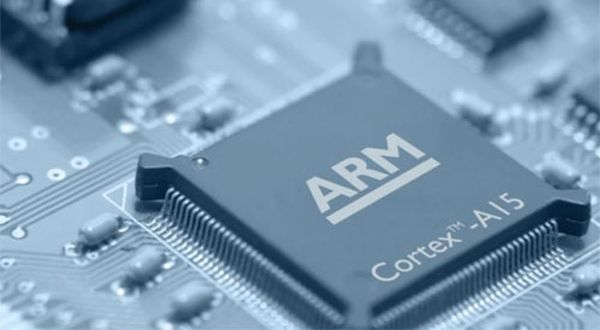
\includegraphics [width =0.6\textwidth]{ARM-Cortex.jpg}
 \end{figure}
 \vspace{-2cm}
 \titlepage
\end{frame}
  
\begin{frame}[t]
 \frametitle{Agenda}
  \footnotesize \tableofcontents
\end{frame}

\definecolor{OliveGreen}{RGB}{2,80,1}
\definecolor{LigthOrange}{RGB}{255,255,200}
\definecolor{gray97}{gray}{.97}
\definecolor{Gray}{RGB}{171,174,178}
\definecolor{orange}{RGB}{255,127,0}

%Comandos para tipografías especiales a nombres relevantes

\AtBeginSubsection[]
{
\begin{frame}{Temario}
\begin{textblock*}{\textwidth}(0.4cm,1.5cm)
%   \begin{multicols}{2}
    \setcounter{tocdepth}{2}  
    \footnotesize \tableofcontents[currentsection, currentsubsection, sectionstyle=show/shaded, subsectionstyle=show/shaded]
%   \end{multicols}
\end{textblock*}
\end{frame}
}

\section{Lenguaje Ensamblador}
\subsection{Estructura de un programa}
\begin{frame}[plain]
 \Large
 \justifying
 \textit{``Simplicity is a great virtue but it requires hard work to achieve it and education to appreciate it. And to make matters worse: complexity sells better.''}
 
 \small
 \begin{flushright}  
  \textit{Edsger Wybe Dijkstra}
 \end{flushright} 
\end{frame}

\begin{frame}[fragile]{Archivo de texto plano con tres campos}
 \begin{textblock*}{\textwidth}(.3cm,1.2cm)
  \begin{onlyenv}<1-5>
   \{label\} \{instrucción \textbar directiva \textbar pseudo-instrucción\} \{;comentario\}
  \end{onlyenv}
 \end{textblock*}
 \begin{textblock*}{\textwidth}(.3cm,1.6cm)
  \begin{onlyenv}<2-5>
   \begin{lstlisting}[escapechar=\@,]
       .section .text ;Nombre de la secci@\color{purple}\'o@n de c@\color{purple}\'o@digo
       .equ  VALUE, 3     
start: MOV  r0, #10   ;Establece los operandos
       LDR  r1, =VALUE;Las constantes literales no llevan #
       ADD  r0,r0,r1  ;r0 = r0 + r1
stop:  WFI            ;Se detiene hasta que llegue una interrupci@\color{purple}\'o@n.
       B   stop       ;Vuelve a esperar interrupci@\color{purple}\'o@n. As@\color{purple}\'i@ se hace un 
                      ;bucle infinito. 
   \end{lstlisting}
  \end{onlyenv}
 \end{textblock*}
 \begin{textblock*}{\textwidth}(.3cm,4.9cm)
  \begin{block}<3->{Campo Instrucción}
   \justifying Se compone a su vez de dos sub campos:
   \begin{itemize}[<+(3)->] \justifying
    \item Código de Operación (\textbf{Opcode}). Siempre existe
    \item Operandos. En ocasiones los operandos no existen o están implícitos en el Opcode
   \end{itemize}
  \end{block}
 \end{textblock*}
\end{frame}

\begin{frame}[fragile]{Archivo de texto plano con tres campos}
 \begin{textblock*}{\textwidth}(.3cm,1.2cm)
  \begin{onlyenv}<1-4>
   \{label\} \{instrucción \textbar directiva \textbar pseudo-instrucción\} \{;comentario\}
  \end{onlyenv}
 \end{textblock*}
 \begin{textblock*}{\textwidth}(.3cm,1.6cm)
  \begin{onlyenv}<1-4>
   \begin{lstlisting}[escapechar=\@,]
       .section .text ;Nombre de la secci@\color{purple}\'o@n de c@\color{purple}\'o@digo
       .equ  VALUE, 3     
start: MOV  r0, #10   ;Establece los operandos
       LDR  r1, =VALUE;Las constantes literales no llevan #
       ADD  r0,r0,r1  ;r0 = r0 + r1
stop:  WFI            ;Se detiene hasta que llegue una interrupci@\color{purple}\'o@n.
       B   stop       ;Vuelve a esperar interrupci@\color{purple}\'o@n. As@\color{purple}\'i@ se hace un 
                      ;bucle infinito. 
   \end{lstlisting}
  \end{onlyenv}
 \end{textblock*}
 \begin{textblock*}{\textwidth}(.3cm,4.9cm)
  \begin{block}{Etiquetas (Labels)}
   \begin{itemize}[<+(1)->] \justifying
    \item Sirven para identificar valores numéricos mediante nombres.
    \item Un valor constante que se define para uso del ensamblador.
    \item Una dirección de memoria que se desea identificar. Puede corresponder a una variable o a una subrutina.
   \end{itemize}
  \end{block}
 \end{textblock*}
\end{frame}

\begin{frame}[fragile]{Archivo de texto plano con tres campos}
 \begin{textblock*}{\textwidth}(.3cm,1.2cm)
  \begin{onlyenv}<1-5>
  \{label\} \{instrucción \textbar directiva \textbar pseudo-instrucción\} \{;comentario\}
  \end{onlyenv}
 \end{textblock*}
 \begin{textblock*}{\textwidth}(.3cm,1.6cm)
  \begin{onlyenv}<1-5>
   \begin{lstlisting}[escapechar=\@,]
       .section .text ;Nombre de la secci@\color{purple}\'o@n de c@\color{purple}\'o@digo
       .equ  VALUE, 3     
start: MOV  r0, #10   ;Establece los operandos
       LDR  r1, =VALUE;Las constantes literales no llevan #
       ADD  r0,r0,r1  ;r0 = r0 + r1
stop:  WFI            ;Se detiene hasta que llegue una interrupci@\color{purple}\'o@n.
       B   stop       ;Vuelve a esperar interrupci@\color{purple}\'o@n. As@\color{purple}\'i@ se hace un 
                      ;bucle infinito. 
   \end{lstlisting}
  \end{onlyenv}
 \end{textblock*}
 \begin{textblock*}{\textwidth}(.3cm,4.9cm)   
  \begin{block}{Instrucciones}
   \begin{itemize}[<+(1)->] \justifying
    \item Son órdenes que el programa le imparte a la CPU.
    \item Mnemónico: Abreviatura de la acción que realiza la instrucción.
    \item Operando(s). Localización o referencia a los valores que requiere la instrucción para ejecutarse y ubicación o referencia del resultado
    \item Puede no haber operando o estar implícito. En tales casos solo hay Mnemónico. 
   \end{itemize}
  \end{block}
 \end{textblock*}
\end{frame}

\begin{frame}[fragile]{Archivo de texto plano con tres campos}
 \begin{textblock*}{\textwidth}(.3cm,1.2cm)
  \begin{onlyenv}<1-5>
   \{label\} \{instrucción \textbar directiva \textbar pseudo-instrucción\} \{;comentario\}
  \end{onlyenv}
 \end{textblock*}
 \begin{textblock*}{\textwidth}(.3cm,1.6cm)
  \begin{onlyenv}<1-5>
   \begin{lstlisting}[escapechar=\@,]
       .section .text ;Nombre de la secci@\color{purple}\'o@n de c@\color{purple}\'o@digo
       .equ  VALUE, 3     
start: MOV  r0, #10   ;Establece los operandos
       LDR  r1, =VALUE;Las constantes literales no llevan #
       ADD  r0,r0,r1  ;r0 = r0 + r1
stop:  WFI            ;Se detiene hasta que llegue una interrupci@\color{purple}\'o@n.
       B   stop       ;Vuelve a esperar interrupci@\color{purple}\'o@n. As@\color{purple}\'i@ se hace un 
                      ;bucle infinito. 
   \end{lstlisting}
  \end{onlyenv}
 \end{textblock*}
 \begin{textblock*}{\textwidth}(.3cm,4.9cm)
  \begin{block}{Directivas}
   \begin{itemize}[<+(1)->] \justifying
    \item No generan código.
    \item Son órdenes para el ensamblador. No para la CPU
    \item Ayudan a definir constantes, variables, e información útil para que el ensamblador ``arme'' la imagen binaria del programa. 
    \item Varían según el ensamblador que utilicemos. En nuestro caso GNU Assembler (\textbf{\textit{as}}).
   \end{itemize}
  \end{block}
 \end{textblock*}
\end{frame}

\begin{frame}[fragile]{Archivo de texto plano con tres campos}
 \begin{textblock*}{\textwidth}(.3cm,1.2cm)
  \begin{onlyenv}<1-4>
   \{label\} \{instrucción \textbar directiva \textbar pseudo-instrucción\} \{;comentario\}
  \end{onlyenv}
 \end{textblock*}
 \begin{textblock*}{\textwidth}(.3cm,1.6cm)
  \begin{onlyenv}<1-4>
   \begin{lstlisting}[escapechar=\@,]
       .section .text ;Nombre de la secci@\color{purple}\'o@n de c@\color{purple}\'o@digo
       .equ  VALUE, 3     
start: MOV  r0, #10   ;Establece los operandos
       LDR  r1, =VALUE;Las constantes literales no llevan #
       ADD  r0,r0,r1  ;r0 = r0 + r1
stop:  WFI            ;Se detiene hasta que llegue una interrupci@\color{purple}\'o@n.
       B   stop       ;Vuelve a esperar interrupci@\color{purple}\'o@n. As@\color{purple}\'i@ se hace un 
                      ;bucle infinito. 
  \end{lstlisting}
 \end{onlyenv}
\end{textblock*}
\begin{textblock*}{\textwidth}(.3cm,4.9cm)   
 \begin{block}{Comentarios}
   \begin{itemize}[<+(1)->] \justifying
    \item No generan código.
    \item Inician con el caracter ';'.
    \item Bien empleados son la documentación de tu proyecto (doxygen por ejemplo).
   \end{itemize}
  \end{block}
 \end{textblock*}
\end{frame}

\begin{frame}[fragile]{Archivo de texto plano con tres campos}
 \begin{textblock*}{\textwidth}(.3cm,1.2cm)
  \begin{onlyenv}<1-4>
   \{label\} \{instrucción \textbar directiva \textbar pseudo-instrucción\} \{;comentario\}
  \end{onlyenv}
 \end{textblock*}
 \begin{textblock*}{\textwidth}(.3cm,1.6cm)
  \begin{onlyenv}<1-4>
   \begin{lstlisting}[escapechar=\@,]
       .section .text ;Nombre de la secci@\color{purple}\'o@n de c@\color{purple}\'o@digo
       .equ  VALUE, 3
start: MOV  r0, #10   ;Establece los operandos
       LDR  r1, =VALUE;Las constantes literales no llevan #
       ADD  r0,r0,r1  ;r0 = r0 + r1
stop:  WFI            ;Se detiene hasta que llegue una interrupci@\color{purple}\'o@n.
       B   stop       ;Vuelve a esperar interrupci@\color{purple}\'o@n. As@\color{purple}\'i@ se hace un
                      ;bucle infinito.
   \end{lstlisting}
  \end{onlyenv}
 \end{textblock*}
 \begin{textblock*}{\textwidth}(.3cm,4.9cm)
  \begin{block}{Ningún campo es obligatorio}
   \begin{itemize}[<+(1)->] \justifying
    \item La línea 8 contiene tan solo un comentario.
    \item Hay solo dos líneas con etiquetas.
    \item Los comentarios van solo donde aplica comentar algo.
   \end{itemize}
  \end{block}
 \end{textblock*}
\end{frame}

\begin{frame}[fragile]{Directivas - Pseudoinstrucciones}
 \begin{textblock*}{\textwidth}(.3cm,1.2cm)
  \begin{itemize}[<+(1)->]\justifying
   \item Definiendo variables\dots
   \setlength\itemsep{1em}
   \item[-] \texttt{.byte}, \texttt{.hword}, \texttt{.word}, \texttt{.quad},
   \item directivas
   \item[-] \verb|.equ|, para definir constantes que después no quedan en el archivo objeto.
   \item[-] \verb|.align|, Deja un espacio de direcciones sin usar hasta la próxima dirección múltiplo del valor que se le establece como argumento.
   \item[-] \verb|.fill|, repite una cantidad de veces la instrucción que le sigue.
   \item expresiones 
   \item [-]\verb|.|, se evalúa en la posición en memoria al principio de la línea que contiene la expresión. Es decir, es la dirección actual en la que se encuentra trabajando \texttt{\textbf{\textit{as}}}.
  \end{itemize}
 \end{textblock*}
\end{frame}

\begin{frame}{Debugger}
 \begin{textblock*}{\textwidth}(.3cm,1.2cm)
  \only<2->{\centering 
\includegraphics[width=.46\textwidth]{debugging.png}}
 \end{textblock*}
\end{frame}

\begin{frame}[fragile]{\texttt{GDB + algún aditivo}}
 \begin{textblock*}{\textwidth}(.3cm,1.2cm)
    Comandos Básicos\\
\small
\begin{tabular}{ll}
\verb;r  | run;            & Ejecuta el programa hasta el primer break\\
& \\
\verb;b  | break FILE:LINE;& Breakpoint en la línea\\
\verb;b  | break FUNCTION; & Breakpoint en la función\\
\verb;info breakpoints;    & Muestra información sobre los breakpoints\\
& \\
\verb;c  | continue;       & Continúa con la ejecución\\
\verb;s  | step;           & Siguiente línea (Into)\\
\verb;n  | next;           & Siguiente línea (Over)\\
\verb;si | stepi;          & Siguiente instrucción asm (Into)\\
\verb;ni | nexti;          & Siguiente instrucción asm (Over)\\
& \\
\verb;x/Nuf ADDR;          & Muestra los datos en memoria\\ % i.e. x/4gx $rsp
  \end{tabular}\\
 \end{textblock*}
 \begin{textblock*}{\textwidth}(.3cm,7.0cm)
  \scriptsize
\hspace{.5cm} \verb;N; = Cantidad (se mide en bytes)\\
\hspace{.5cm} \verb;u; = Unidad \verb;b(byte), h(half word), w(word), g(giant, 8-bit)|;\\
\hspace{.5cm} \verb;f; = Formato \verb;x(hex), d(decimal), u(unsigned decimal), o(octal), f(float), a(address);\\
\hspace{2.1cm} \verb;t:binary, i(instruction), c(char), s(string), z(hex, zero padded on the left);\\
 \end{textblock*}
\end{frame}

\begin{frame}[fragile]{GDB}
Configuración de GDB:\\
\vspace{0.1cm}
\begin{verbatim}
    ~/.gdbinit 
\end{verbatim}
\vspace{0.4cm}
Para usar sintaxis intel y guardar historial de comandos:\\
\vspace{0.1cm}
\begin{verbatim}
    set disassembly-flavor intel
    set history save
\end{verbatim}
\vspace{0.4cm}
Correr \texttt{GDB} con argumentos:
\vspace{0.1cm}
\begin{verbatim}
    gdb --args <ejecutable> <arg1> <arg2> ...
\end{verbatim}
\end{frame}

\section{ABI: Aplication Binary Interface}
\subsection{Pila y Convención C}
\begin{frame}{¿Que es ABI?}
 \begin{textblock*}{\textwidth}(.3cm,1.0cm)
  \begin{block}<2->{\textbf{ABI} (\textbf{A}pplication \textbf{B}inary \textbf{I}nterface)}
   \justifying Es la especificación de una convención de llamadas entre dos módulos de Software, a nivel de lenguaje de máquina, fundamental para interfacear llamadas a funciones de bajo nivel desde lenguajes de alto nivel o viceversa, e imprescindible para que puedan diseñarse compiladores de lenguajes que trabajen de un modo predecible.
  \end{block}
 \end{textblock*}
 \begin{textblock*}{\textwidth}(.3cm,3.7cm) 
  \begin{itemize}[<+(2)->]\justifying 
   \item De esta forma las funciones pueden ser llamadas sin tener en cuenta como fueron implementadas.
   \item La convención define:
   \begin{itemize}
    \item[$\checkmark$] Como las funciones reciben parámetros.
    \item[$\checkmark$] Como las funciones retornan el resultado.
    \item[$\checkmark$] Que registros se deben preservar en una función.
   \end{itemize}
   \item Las convenciones dependen de la arquitectura del procesador:
   \begin{itemize}
    \item[$\checkmark$] En \texttt{x86} (\SI{32}{\bit}) se conoce como \texttt{x32 ABI}.
    \item[$\checkmark$] En \texttt{x86-64} (\SI{64}{\bit}) se denomina \texttt{System V AMD64 ABI}.
    \item[$\checkmark$] En \texttt{ARMv7} es la \texttt{Procedure Call Standard for the Arm Architecture}.
   \end{itemize}
  \end{itemize}
 \end{textblock*}
\end{frame}

\begin{frame}{Tipos de Datos Fundamentales}
 \begin{textblock*}{\textwidth}(.3cm,1.2cm)
  \centering 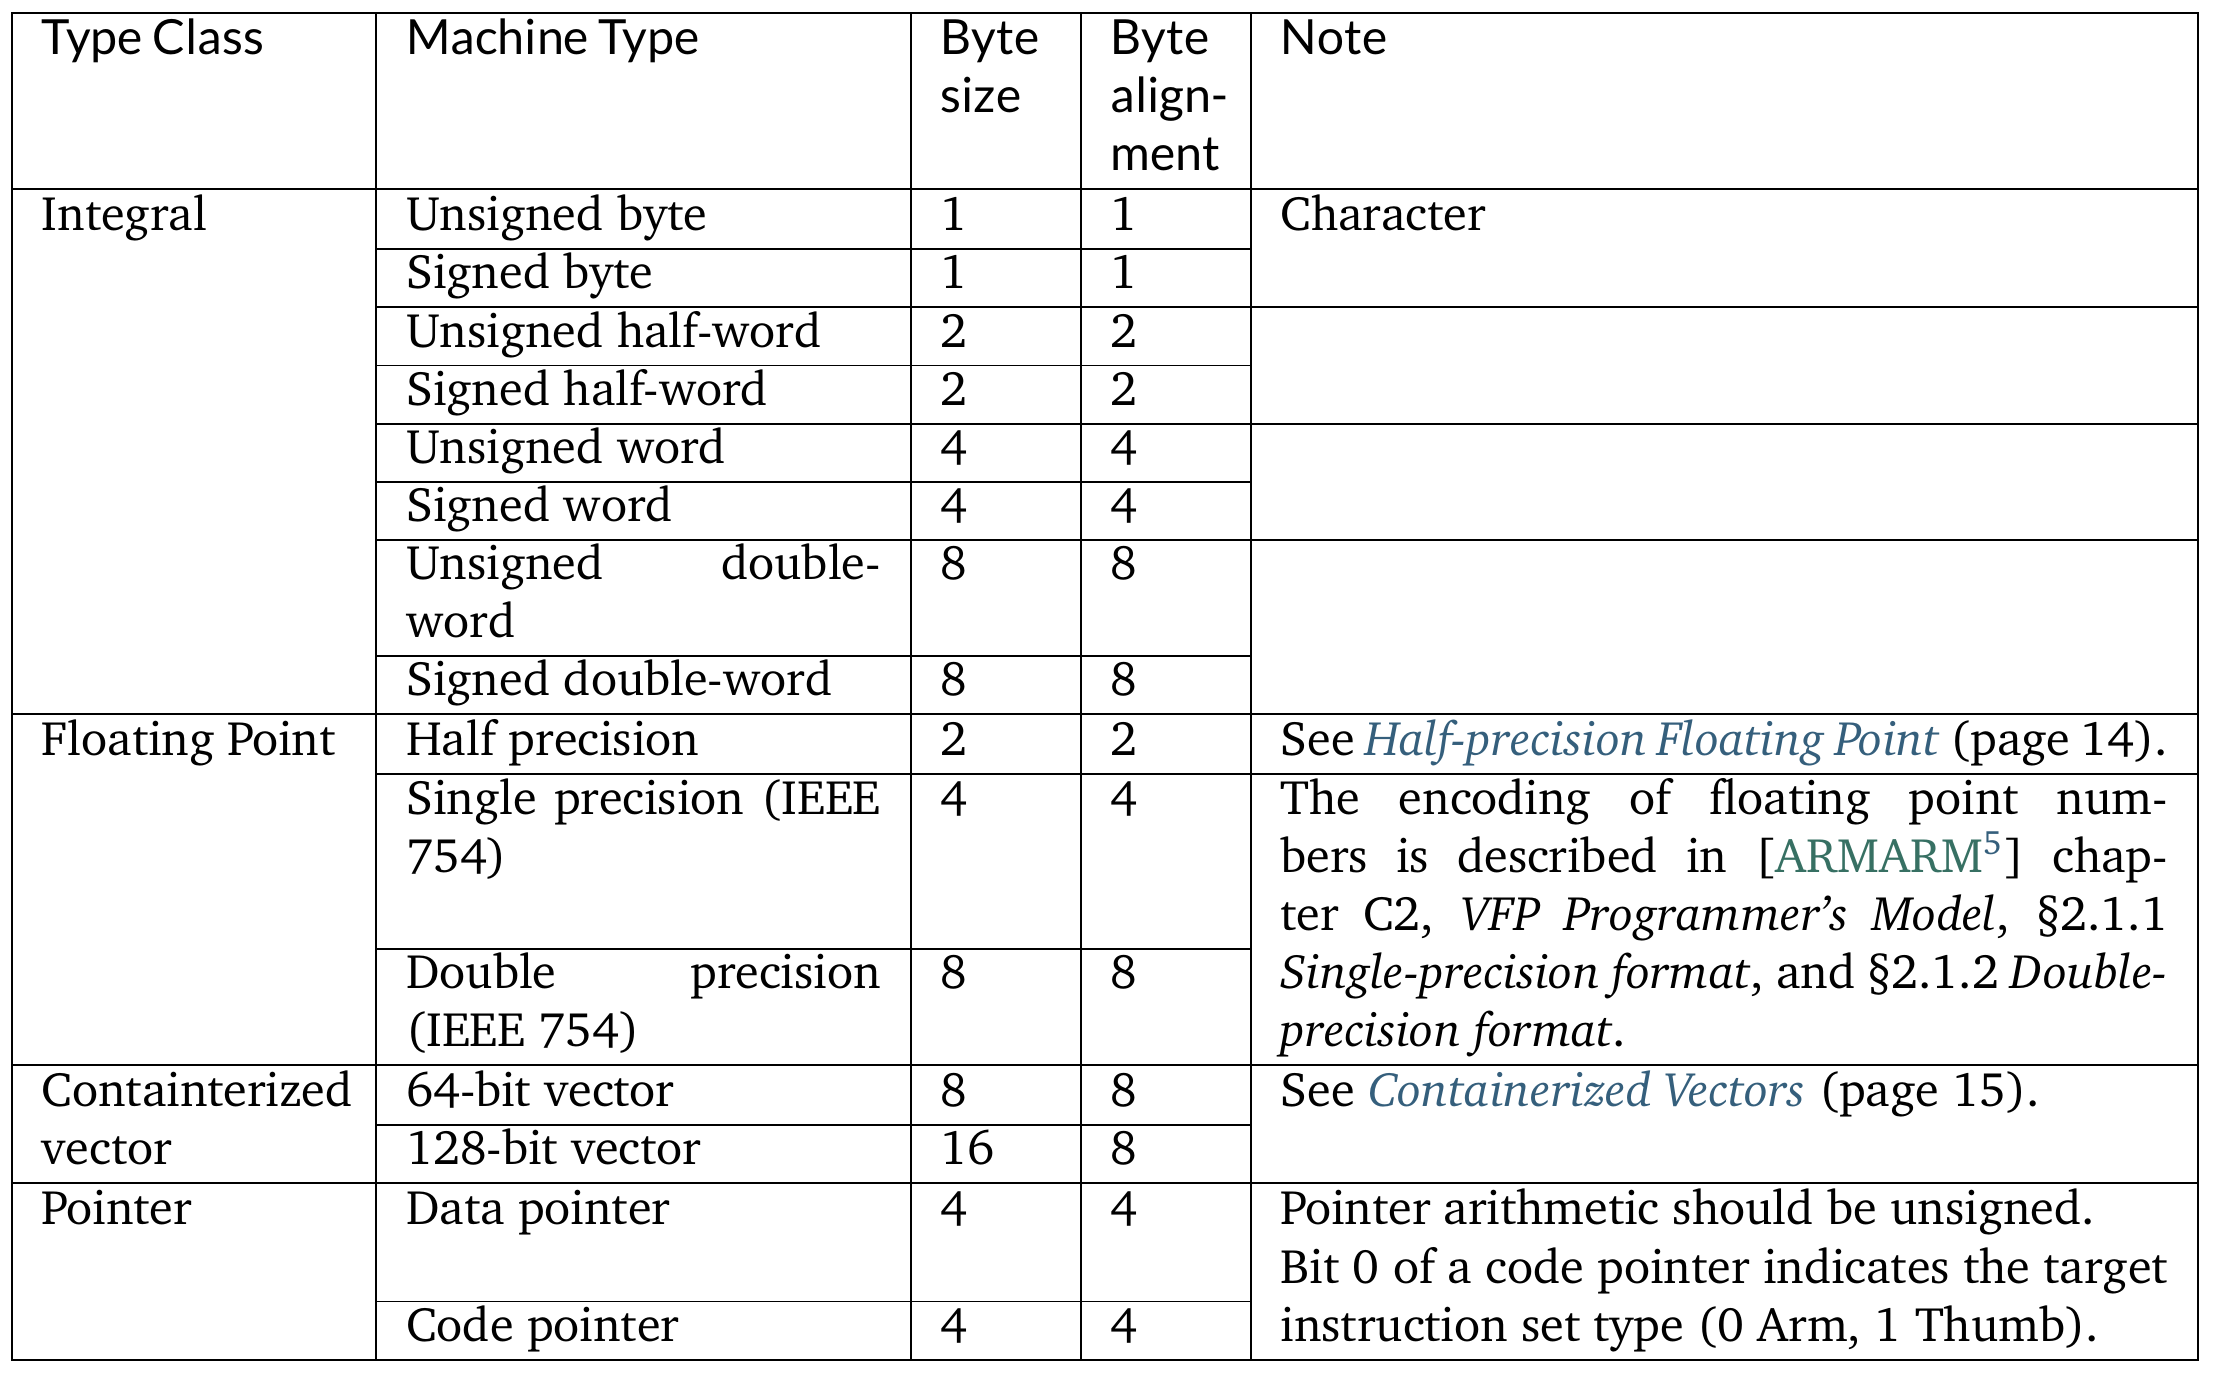
\includegraphics[width=.77\textwidth]{FDT.png}
 \end{textblock*}
\end{frame}

\begin{frame}{Uso de los registros}
 \begin{textblock*}{\textwidth}(.3cm,1.2cm)
 \begin{scriptsize}
  \begin{center}
   \begin{tikzpicture}
    \node (tbl1) { 
    \rowcolors[]{1}{}{gray!5}
     \begin{tabularx}{.765\textwidth}{l c c l } %{p{.05\textwidth} p{.2\textwidth} p{.2\textwidth} p{.45\textwidth} }
 \textbf{\color{white} Reg.} & \textbf{\color{white} Alias} & \textbf{\color{white} Especial} & \textbf{ \color{white} Rol en la llamada}\\
  R0 & arg1 & & Registro scratch Argumento 1 / resultado\\
  R1 & arg2 & & Registro scratch Argumento 2 / resultado\\
  R2 & arg3 & & Registro scratch Argumento 3\\
  R3 & arg4 & & Registro scratch Argumento 4\\
  R4 & var1 & & Registro variable 1\\
  R5 & var2 & & Registro variable 2\\
  R6 & var3 & & Registro variable 3\\
  R7 & var4 & & Registro variable 4\\
  R8 & var5 & & Registro variable 5\\
  R9 & v6 SB TR & & Platform defined \\    
  R10 & var7 & & Registro variable 7\\    
  R11 & var8 & FP & Frame Pointer o Variable 8\\    
  R12 & & IP & Intra Procedure Call Scratch Register\\
  R13 & & SP & Stack Pointer\\
  R14 & & LR & Link Register\\    
  R15 & & PC & Program Counter\\    
     \end{tabularx}
    };
    \begin{pgfonlayer}{background}
     \draw[rounded corners,top color=blue,bottom color=black,draw=white] ($(tbl1.north west)+(0.14,0)$) rectangle ($(tbl1.north east)-(2,0.45)$);
     \draw[rounded corners,top color=white,bottom color=black, middle color=blue,draw=blue!20] ($(tbl1.south west)+(0.12,0.5)$) rectangle ($(tbl1.south east)-(2,0)$);
     \draw[top color=blue!1,bottom color=blue!20,draw=white] ($(tbl1.north east)-(2,0.6)$) rectangle ($(tbl1.south west)+(0.13,0.2)$);
    \end{pgfonlayer}
   \end{tikzpicture}
  \end{center}
 \end{scriptsize}
\end{textblock*}
\end{frame}

\begin{frame}{ABI. Tratamiento de los registros de extensiones}
 \begin{textblock*}{\textwidth}(.3cm,1.2cm)
  \begin{itemize}[<+(1)->] \justifying \parskip 0.5cm
   \item Los registros \texttt{\textbf{s0}} a \texttt{\textbf{s15}}, (o \textbf{\texttt{d0}} a \texttt{\textbf{d7}}, o \textbf{\texttt{q0}} a \textbf{\texttt{q3}}), no se preservan y pueden ser utilizados para pasaje de argumentos o retorno de resultados en las variantes de procedure call standards.
   \item Deben ser preservados los registros \texttt{\textbf{s16}} a \texttt{\textbf{s31}} (o \textbf{\texttt{d8}} a \texttt{\textbf{d15}}, o \textbf{\texttt{q4}} a \textbf{\texttt{q7}}).
   \item De estar presentes, los registros \textbf{\texttt{d16}} a \texttt{\textbf{d31}}, (o \textbf{\texttt{q8}} a \textbf{\texttt{q15}}), no necesitan ser preservados.
  \end{itemize}
 \end{textblock*}
\end{frame}

\begin{frame}{La pila en llamadas a procedimientos}
 \begin{textblock*}{\textwidth}(.3cm,1.2cm)
  \begin{itemize}[<+(1)->] \justifying  \parskip 0.5cm
   \item ARM define restricciones a observar en el uso de la pila, algunas son de mínima y se amplían cuando se pretende universalizar la interfaz de programación (ABI).
   \item El Stack debe ser un área contigua y es \textbf{\textit{full descending}}: Esto significa que crece desde una Dirección Base hacia una Dirección Tope
   \item Alineación: ARM define dos criterios:
   \begin{description}[Restricción Interfaz Pública] \justifying \parskip 0.5cm
    \item[Restricción Universal] sp mod 4 = 0        %\hskip 2cm
    \item[Restricción Interfaz Pública] sp mod 8 = 0 %\hskip 1cm
   \end{description}
  \end{itemize}
 \end{textblock*}
\end{frame}

\begin{frame}{Stack frame}
 \begin{textblock*}{\textwidth}(.3cm,1.2cm)
  \begin{itemize}[<+(1)->] \justifying
   \item Sabemos a esta altura que una función en C es ejecutada dentro de un \textbf{scope}, en el cual tienen validez sus variables locales así como los argumentos que recibe de la función invocante.
   \item Esto se debe a una estructura fundamental.
   \item[] \begin{block}<3->{stack frame}
    \justifying Estructura en memoria constituida por el conjunto de registros preservados, las variables locales y los argumentos pasados desde la función invocante, eventualmente la dirección de retorno (en el caso de ARM no aplica), y una referencia al siguiente Stack Frame en caso de llamadas anidadas.
    \end{block}
   \vspace{-0.5cm}
   \item La construcción del \emph{stack frame} consiste en colocar un registro puntero en una dirección relativa al comienzo del frame en el stack de la función invocante. Este se denomina \textbf{Frame Pointer}.
   \item No se especifica el lugar exacto del Stack Frame en el que se ubica el Frame Pointer
  \end{itemize}
 \end{textblock*}
\end{frame}

\begin{frame}{Llamada}
 \begin{textblock*}{\textwidth}(.3cm,1.2cm)
  \begin{itemize}[<+(1)->] \justifying \parskip 0.15cm
   \item ARMv7 usa la instrucción \textbf{BL} (\textbf{B}ranch with \textbf{L}ink).
   \item Para comenzar a ejecutar \textbf{BL}, la CPU transfiere a \textbf{\texttt{LR[31:1]}} los 31 MSB de la dirección de la instrucción sucesora secuencial (es decir, la que sigue a BL en la secuencia de instrucciones del programa). 
   \item El valor del LSB, \textbf{\texttt{LR[0]}} se establecerá de acuerdo con el Modo en que esté el procesador: Será \textbf{\texttt{LR[0]='1'}} si el procesador trabaja en Modo \Thumb, o \textbf{\texttt{LR[0]='0'}} si está en Modo \arm.
   \item Acto seguido, se escribe en el Program Counter el valor de la dirección de salto contenida en la instrucción. Los rangos de salto dependen del modo de trabajo.
   \begin{description}[Modo \Thumb-2] \parskip 0.15cm
    \item [Modo \arm] \textpm \SI{32}{\mebi\byte}
    \item [Modo \Thdos] \textpm \SI{16}{\mebi\byte}
    \item [Modo \Thumb] \textpm \SI{4}{\mebi\byte}
   \end{description}
  \end{itemize}
 \end{textblock*}
\end{frame}

\begin{frame}{Pasaje de argumentos}
 \begin{textblock*}{\textwidth}(.3cm,1.2cm)
  \begin{itemize}[<+(1)->] \justifying %\parskip 0.15cm
   \item El estándar base establece que el proceso invocante utilice los registros core \textbf{\texttt{[R0:R3]}} para pasar los primeros argumentos al proceso invocado. 
   \item Utilizará solo los que necesite iniciando por \textbf{\texttt{R0}} para el 1er. argumento.
   \item En caso que no resulten suficientes en virtud de los argumentos que se necesita enviar, deberá continuar su envío utilizando el stack.
   \item Un considerable porcentaje de funciones invocantes utilizan pocos argumentos, y por lo tanto puede ser satisfecho con estos 4 registros. 
   \item De este modo el procesador logra resolver el pasaje con overhead mínimo.
   \item La pila no posee limitaciones de cantidad de argumentos pero penaliza claramente la performance ya que cada operación involucra memoria.
   \item Si la CPU soporta extensiones de arquitectura (punto flotante por ejemplo), entonces de acuerdo al tipo de dato fundamental de cada parámetro puede utilizarse un registro core o uno de un coprocesador que implemente la extensión de arquitectura.
  \end{itemize}
 \end{textblock*}
\end{frame}

\begin{frame}{Pasaje de argumentos}
 \begin{textblock*}{\textwidth}(.3cm,1.2cm)
  \begin{itemize}[<+->] \justifying \parskip 0.3cm
   \item Si el argumento es un tipo de dato compuesto cuyo tamaño no puede ser determinado, la función invocante debe tenerlo almacenado previamente en memoria, \textbf{alineado a \SI{4}{\byte}}, y enviará como argumento un puntero en el próximo registro core disponible (o eventualmente en la pila si éstos se hubieren agotado).
   \item Si el argumento es un tipo de dato compuesto cuyo tamaño no es múltiplo de 4, su tamaño se lleva al múltiplo de 4 inmediato superior.
   \item Tipos fundamentales de datos con tamaño menor de \SI{4}{\byte}, pasan en la parte menos significativa del registro correspondiente (o de la posición de la pila en su defecto), con la extensión de signo o cero que corresponda al tipo de dato.
  \end{itemize}
 \end{textblock*}
\end{frame}

\begin{frame}{Pasaje de argumentos}
 \begin{textblock*}{\textwidth}(.3cm,1.2cm)
  \begin{itemize}[<+->] \justifying \parskip 0.3cm
   \item Un Tipo de Dato Fundamental (\textbf{TDF}) que requiere alineación a \SI{8}{\byte} se almacena a partir de un Registro par, o en caso de estar en la pila con ese alineamiento.
   \item Si el tamaño en words del \textbf{TDF} no cabe en la cantidad de Registros disponibles, el argumento se divide parte en el Registro Core \textbf{hasta completar R3}, y la otra parte pasa por la pila.
  \end{itemize}
 \end{textblock*}
\end{frame}

\begin{frame}{Pasaje de argumentos con coprocesadores activos}
 \begin{textblock*}{\textwidth}(.3cm,1.2cm)
  \begin{itemize}[<+(1)->]
   \item Half Presicion -\textgreater Parte baja de un Registro Sn. ($0 \leqslant n \leqslant 15$)
   \item Single Presicion -\textgreater Registro Sn ($0 \leq n \leq 15$).
   \item Double Presicion -\textgreater Registro Di ($0 \leq i \leq 7$).
   \item Vector Empaquetado en \SI{64}{\bit} -\textgreater Registro Di ($0 \leq i \leq 7$).
   \item Vector Empaquetado en \SI{128}{\bit} -\textgreater Registro Qj ($0 \leq j \leq 3$).
  \end{itemize}
 \end{textblock*}
\end{frame}

\begin{frame}{Retorno de resultados base}
 \begin{textblock*}{\textwidth}(.3cm,1.2cm)
  \only<1->{En general se utilizan los registros \textbf{\texttt{[R0:R3]}}, dependiendo del tamaño del resultado.}
  \begin{itemize}[<+(1)->] \justifying \parskip 0.2cm
   \item Half Precision Floating Point: \textbf{\texttt{R0[15:0]}}.
   \item Tipo de dato Fundamental menor de \SI{4}{\byte}: \textbf{\texttt{R0}} con extensión de signo.
   \item Tipo de dato Fundamental de \SI{4}{\byte} (int o float por ejemplo): \textbf{\texttt{R0}}.
   \item Tipo de dato Fundamental de \SI{8}{\byte} (long long, double, o vectores de \SI{8}{\byte}): \textbf{\texttt{[R0:R1]}}.
   \item Vector de \SI{16}{\byte}: \textbf{\texttt{[R0:R3]}}.
   \item Tipo de dato compuesto menor de \SI{4}{\byte}: \textbf{\texttt{R0}}.
   \item Tipo de dato de tamaño indeterminado: Se almacena en memoria alineado a \SI{4}{\byte} y se pasa su referencia por \textbf{\texttt{R0}}.
  \end{itemize}
 \end{textblock*}
\end{frame}

\begin{frame}{Retorno de resultados con coprocesadores activos}
 \begin{textblock*}{\textwidth}(.3cm,1.2cm) 
  \begin{itemize}[<+(1)->] \justifying \parskip 0.5cm
   \item En general si está habilitado el coprocesador los valores de punto flotante o datos SIMD empaquetados retornan por el registro \textbf{\texttt{S0}}, \textbf{\texttt{D0}}, ó \textbf{\texttt{Q0}}, según el Tipo de Dato Fundamental que se trate.
   \item El resto del los Tipos de Datos Fundamentales se retornan de la manera definida en el estándar base. 
  \end{itemize}
 \end{textblock*}
\end{frame}

\begin{frame}{Ejemplo 1}
 \begin{textblock*}{\textwidth}(.3cm,1.5cm) 
  \textbf{\texttt{int f1( int a, float b, double c, int* d, double* e)}}\\
 \end{textblock*}
 \begin{textblock*}{\textwidth}(0.5cm,2.5cm) \only<1>{\centering \includegraphics[scale=0.55]{ejemplo64-1-layer1.pdf}} \end{textblock*}
 \begin{textblock*}{\textwidth}(0.5cm,2.5cm) \only<2>{\centering \includegraphics[scale=0.55]{ejemplo64-1-layer2.pdf}} \end{textblock*}
 \begin{textblock*}{\textwidth}(0.5cm,2.5cm) \only<3>{\centering \includegraphics[scale=0.55]{ejemplo64-1-layer3.pdf}} \end{textblock*}
 \begin{textblock*}{\textwidth}(0.5cm,2.5cm) \only<4>{\centering \includegraphics[scale=0.55]{ejemplo64-1-layer4.pdf}} \end{textblock*}
 \begin{textblock*}{\textwidth}(0.5cm,2.5cm) \only<5>{\centering \includegraphics[scale=0.55]{ejemplo64-1-layer5.pdf}} \end{textblock*}
 \begin{textblock*}{\textwidth}(0.5cm,2.5cm) \only<6>{\centering \includegraphics[scale=0.55]{ejemplo64-1-layer6.pdf}} \end{textblock*}
%  \begin{textblock*}{\textwidth}(0.5cm,2.5cm) \only<7>{\centering \includegraphics[scale=0.55]{img/ejemplo64-1-7.pdf}} \end{textblock*}
\end{frame}

\begin{frame} {Ejemplo 1}
 \begin{textblock*}{\textwidth}(.3cm,1.5cm) 
  \textbf{\texttt{int f1( int a, float b, double c, int* d, double* e)}}\\
 \end{textblock*}
 \begin{textblock*}{\textwidth}(0.5cm,2.5cm) \only<1>{\centering \includegraphics[scale=0.55]{ejemplo64-1b-layer1.pdf}} \end{textblock*}
 \begin{textblock*}{\textwidth}(0.5cm,2.5cm) \only<2>{\centering \includegraphics[scale=0.55]{ejemplo64-1b-layer2.pdf}} \end{textblock*}
 \begin{textblock*}{\textwidth}(0.5cm,2.5cm) \only<3>{\centering \includegraphics[scale=0.55]{ejemplo64-1b-layer3.pdf}} \end{textblock*}
 \begin{textblock*}{\textwidth}(0.5cm,2.5cm) \only<4>{\centering \includegraphics[scale=0.55]{ejemplo64-1b-layer4.pdf}} \end{textblock*}
 \begin{textblock*}{\textwidth}(0.5cm,2.5cm) \only<5>{\centering \includegraphics[scale=0.55]{ejemplo64-1b-layer5.pdf}} \end{textblock*}
 \begin{textblock*}{\textwidth}(0.5cm,2.5cm) \only<6>{\centering \includegraphics[scale=0.55]{ejemplo64-1b-layer6.pdf}} \end{textblock*}
\end{frame}

\begin{frame}{Ejemplo insano (solo para mostrar que el ABI resiste lo que sea....)}
 \begin{textblock*}{\textwidth}(.3cm,1.2cm) 
  \textbf{\texttt{int f( int a1, float a2, double a3, int a4, float a5, double a6, int* a7, double* a8, int* a9, double a10, int** a11, float* a12, double** a13, int* a14, float a15)}}
 \end{textblock*}
 \begin{textblock*}{\textwidth}(0.5cm,2.5cm) \only<1>{\centering \includegraphics[scale=0.55]{ejemplo64-2-layer1.pdf}} \end{textblock*}
 \begin{textblock*}{\textwidth}(0.5cm,2.5cm) \only<2>{\centering \includegraphics[scale=0.55]{ejemplo64-2-layer2.pdf}} \end{textblock*}
 \begin{textblock*}{\textwidth}(0.5cm,2.5cm) \only<3>{\centering \includegraphics[scale=0.55]{ejemplo64-2-layer3.pdf}} \end{textblock*}
 \begin{textblock*}{\textwidth}(0.5cm,2.5cm) \only<4>{\centering \includegraphics[scale=0.55]{ejemplo64-2-layer4.pdf}} \end{textblock*}
 \begin{textblock*}{\textwidth}(0.5cm,2.5cm) \only<5>{\centering \includegraphics[scale=0.55]{ejemplo64-2-layer5.pdf}} \end{textblock*}
 \begin{textblock*}{\textwidth}(0.5cm,2.5cm) \only<6>{\centering \includegraphics[scale=0.55]{ejemplo64-2-layer6.pdf}} \end{textblock*}
 \begin{textblock*}{\textwidth}(0.5cm,2.5cm) \only<7>{\centering \includegraphics[scale=0.55]{ejemplo64-2-layer7.pdf}} \end{textblock*}
 \begin{textblock*}{\textwidth}(0.5cm,2.5cm) \only<8>{\centering \includegraphics[scale=0.55]{ejemplo64-2-layer8.pdf}} \end{textblock*}
 \begin{textblock*}{\textwidth}(0.5cm,2.5cm) \only<9>{\centering \includegraphics[scale=0.55]{ejemplo64-2-layer9.pdf}} \end{textblock*}
 \begin{textblock*}{\textwidth}(0.5cm,2.5cm) \only<10>{\centering \includegraphics[scale=0.55]{ejemplo64-2-layer10.pdf}} \end{textblock*}
 \begin{textblock*}{\textwidth}(0.5cm,2.5cm) \only<11>{\centering \includegraphics[scale=0.55]{ejemplo64-2-layer11.pdf}} \end{textblock*}
 \begin{textblock*}{\textwidth}(0.5cm,2.5cm) \only<12>{\centering \includegraphics[scale=0.55]{ejemplo64-2-layer12.pdf}} \end{textblock*}
 \begin{textblock*}{\textwidth}(0.5cm,2.5cm) \only<13>{\centering \includegraphics[scale=0.55]{ejemplo64-2-layer13.pdf}} \end{textblock*}
 \begin{textblock*}{\textwidth}(0.5cm,2.5cm) \only<14>{\centering \includegraphics[scale=0.55]{ejemplo64-2-layer14.pdf}} \end{textblock*}
 \begin{textblock*}{\textwidth}(0.5cm,2.5cm) \only<15>{\centering \includegraphics[scale=0.55]{ejemplo64-2-layer15.pdf}} \end{textblock*}
 \begin{textblock*}{\textwidth}(0.5cm,2.5cm) \only<16>{\centering \includegraphics[scale=0.55]{ejemplo64-2-layer16.pdf}} \end{textblock*}
\end{frame}

\section{Set de Instrucciones}
\subsection{Conceptos preliminares}
\begin{frame}{Un poco de práctica antes de seguir}
 \begin{textblock*}{\textwidth}(.3cm,1.2cm) 
  \begin{block}{Ejercicio Nro.1}
   Muestre cómo se almacenan en memoria los siguientes datos en procesadores Big-Endian y Little-Endian:
   \begin{center}
    \begin{tabular}{ll}
\texttt{.byte 0x12}           & \texttt{.word 0x12345678}            \\
\texttt{.byte 0x12, 0x34}      & \texttt{.word 0x12345678, 0x9ABCDEF1} \\
\texttt{.hword 0x1234}         & \texttt{.quad 0x123456789ABCDEF1}    \\
\texttt{.hword 0x1234, 0x5678}  & \texttt{.byte \textquotesingle 1\textquotesingle,\textquotesingle 2\textquotesingle,\textquotesingle 3\textquotesingle,\textquotesingle 4\textquotesingle} \\
    \end{tabular}
   \end{center}
  \end{block}
 \end{textblock*}
 \begin{textblock*}{\textwidth}(.3cm,5.8cm) 
  \begin{description}[<+(1)->] [Little Endian] \justifying
   \item[Big Endian]: el byte más significativo en la posición de memoria menos significativa.
   \item[Little Endian]: el byte más significativo en la posición de memoria más significativa.
  \end{description}
 \end{textblock*}
\end{frame}

\begin{frame}{Ejercicio Nro.1. Respuestas}
\small
  \begin{tabular}{ll}
\scriptsize \texttt{.byte 0x12}            &\texttt{-|12|-}\scriptsize big endian \\        
                               &\texttt{-|12|-}\scriptsize little endian  \\
\hline
\scriptsize \texttt{.byte 12h, 0x34}       &\texttt{-|12|34|-}\scriptsize big endian \\        
                               &\texttt{-|12|34|-}\scriptsize little endian  \\  
                                  \hline
\scriptsize \texttt{.hword 0x1234}         &\texttt{-|12|34|-}\scriptsize big endian \\      
                               &\texttt{-|34|12|-}\scriptsize little endian  \\    
                                  \hline
\scriptsize \texttt{.hword 1234h, 0x5678}  &\texttt{-|12|34|56|78|-}\scriptsize big endian \\      
                               &\texttt{-|34|12|78|56|-}\scriptsize little endian  \\    
                                  \hline
\scriptsize \texttt{.word 0x12345678}      &\texttt{-|12|34|56|78|-}\scriptsize big endian \\      
                               &\texttt{-|78|56|34|12|-}\scriptsize little endian  \\    
                                  \hline
\scriptsize \texttt{.word 0x12345678,0x9ABCDEF1}&\texttt{-|12|34|56|78|9A|BC|DE|F1|-}\scriptsize big endian \\      
                                &\texttt{-|78|56|34|12|F1|DE|BC|9A|-}\scriptsize little endian  \\    
                                   \hline
\scriptsize \texttt{.quad 0x123456789ABCDEF1}&\texttt{-|12|34|56|78|9A|BC|DE|F1|-}\scriptsize big endian \\      
                                 &\texttt{-|F1|DE|BC|9A|78|56|34|12|-}\scriptsize little endian  \\    
                                   \hline
\scriptsize \texttt{.byte \textquotesingle 1\textquotesingle,\textquotesingle 2\textquotesingle,\textquotesingle 3\textquotesingle,\textquotesingle 4\textquotesingle}&\texttt{-|31|32|33|34|-}\scriptsize big endian \\
    &\texttt{-|31|32|33|34|-}\scriptsize little endian  \\
 \end{tabular}
\end{frame}

\begin{frame}[t]{Aritmética}
  \begin{block}{Ejercicio Nro.2: Rangos de Representación}
  ¿Cuál es el rango de representación de los números enteros sin signo de 8, 16 y \SI{32}{\bit}?\\
  ¿Cuál es el rango de representación de los números enteros con signo en complemento a dos de 8, 16 y \SI{32}{\bit}?
  \end{block}
  \pause
  \begin{center}
  \begin{tabular}{l|c}
  Sin signo & $0$ a $2^{n}-1$        \\ \hline
  Con signo & $-2^{n-1}$ a $2^{n-1}-1$ \\
  \end{tabular}
  \end{center}
  \begin{center}
  \begin{tabular}{c|c|c}
   & Sin signo & Con signo \\ \hline
    8  & $0$ a $255$         & $-128$ a $127$               \\ \hline
    16 & $0$ a $65535$       & $-32768$ a $32767$           \\ \hline
    32 & $0$ a $4294967295$  & $-2147483648$ a $2147483647$ \\ 
  \end{tabular}
  \end{center}
\end{frame}

\begin{frame}[t,fragile]{Aritmética}
  \begin{block}{Ejercicio Nro.3:}
  \begin{itemize}[<+(1)->]
   \justifying
   \item Expresar los números 133 y 123 en notación binaria de \SI{8}{\bit} (notación sin signo)
   \item Sumar ambos números bit a bit
   \item Expresar los números -123 y 123 en notación complemento a dos de \SI{8}{\bit} y sumarlos bit a bit.
   \item ¿Qué conclusión se puede sacar observando el resultados de ambas operaciones?
  \end{itemize}
  \end{block}
\end{frame}

\begin{frame}[t,fragile]{Aritmética}
Resultado Ejercicio Nro. 3:
\begin{center}
  \begin{tabular}{lp{1cm}l}
  \verb| 123 = 01111011| & & \verb| 123 = 01111011| \\
  \verb|-123 = 10000101| & & \verb| 133 = 10000101| \\
  \cline{1-1} \cline{3-3}
  \verb|      100000000| & & \verb|      100000000| \\
  \end{tabular}
  \end{center}
\begin{itemize}[<+(1)->] \justifying \parskip 1cm 
  \item Esa es la razón por la cual no hay una instrucción para sumar enteros signados y otra diferente para enteros no signados. Lo mismo para la resta. La representación en Ca2 de los números negativos asegura esta propiedad 
  \item \textbf{Es responsabilidad del programador saber con qué tipo de números se está operando, y prestar atención a los flags adecuados.}
\end{itemize}
\end{frame}

\subsection{Instrucciones ARM, Thumb, Thumb-2(T32)}
\begin{frame}{Modos e instrucciones}
 \begin{textblock*}{\textwidth}(.3cm,1.2cm) 
  \begin{itemize}[<+(1)->] \justifying
   \item En ARM7TDMI, se planteó un set de instrucciones de \SI{32}{\bit} de ancho.
   \item Sin embargo introdujo el modo Thumb como un Subset de las instrucciones ARM.
   \begin{itemize} \justifying
    \item [-] \textbf{Trabajan con datos de \SI{32}{\bit} como las ARM}.
    \item [-] Su tamaño es de \SI{16}{\bit} (la mitad)
    \item [-] Su funcionalidad es acotada respecto de las ARM.
   \end{itemize}
   \item Por lo tanto, hay cambios en la sintaxis:
   \begin{description}
    \item[  ARM] \textbf{\texttt{ADD R1,R1,R6}}. Conocido coo formato de tres operandos.
    \item[Thumb] \textbf{\texttt{ADD R1,R6}}
   \end{description}
   \item En Modo \Thumb{} el primer operando es al mismo tiempo el operando destino. Siempre se destruye el primer operando origen.
   \item En Modo \arm{} se conserva el primer operando reemplazando el registro resultado por otro diferente de los dos registros operando origen.
   \item Aquí tenemos un primer caso de perdida de funcionalidad en el Modo \Thumb. Y una ambigüedad para el compilador.
  \end{itemize}
 \end{textblock*}
\end{frame}

\begin{frame}{Unified Assembler Language (\textbf{\textit{UAL}})}
 \begin{textblock*}{\textwidth}(.3cm,1.2cm) 
  \begin{itemize}[<+(1)->] \justifying
   \item Unified Assembler Language (\textbf{\textit{UAL}}) es una sintaxis común para instrucciones \arm{} y \Thumb{}. Reemplaza las versiones anteriores de los lenguajes ensamblador \arm{} y \Thumb{}.
   \item Usando \textbf{\textit{UAL}}, se puede codear para Modo \arm{} o \Thumb{} para cualquier procesador. Eventualmente el ensamblador solucionará el uso de una instrucción inválida.
   \item Desde la Versión ARMv4T, los compiladores soportan \textbf{\textit{UAL}}. Desde entonces, el compilador espera que se programe en \textbf{\textit{UAL}}. 
   \item No obstante se puede especificar el modo en el programa fuente mediante las directivas adecuadas de cada ensamblador, como así también mediante opciones por línea de comandos al compilar.
  \end{itemize}
\end{textblock*}
\end{frame}

\begin{frame}{Unified Assembler Language (\textbf{\textit{UAL}})}
  \begin{textblock*}{\textwidth}(.3cm,1.2cm) 
    \begin{center}
    \begin{tabular}{ll}
     \textbf{Formato \arm/\Thumb}     & \textbf{Formato UAL}\\
     \hline\hline
     STMFD sp!, {reglist}  & POP \{cond\}\{reglist\}\\
     LDMFD sp!,\{reglist\} & PUSH \{cond\}\{reglist\}\\
     \hline
      & MOV Rd, Rn, LSL shift\\
      & MOV Rd, Rn, LSR shift\\
      & MOV Rd, Rn, ASR shift\\
      & MOV Rd, Rn, ROR shift\\
      & MOV Rd, Rn, RRX shift\\
      \hline
      & LDR Rd, [pc, \#offset]\\
      \hline
      ADD r1, r1, r3 & ADD r1, r3\\
    \end{tabular}
  \end{center}
 \end{textblock*}
\end{frame}


\subsection{Ejecución condicional}
\begin{frame}{Ejecución condicional para evitar saltos}
 \begin{textblock*}{\textwidth}(.3cm,1.2cm) 
  \begin{block}<1->{Ventajas de la ejecución condicional}
   \begin{itemize}[<+(1)->] \justifying
    \item Evitar un salto es quitar la instrucción que eventualmente evalúa la condición y de acuerdo a ello salta. Esta quita ya mejora la compresión del código.
    \item Las instrucciones condicionales se ejecutan si la condición establecida es \textbf{\texttt{TRUE}}.
    \item De lo contrario ejecutan No Operate, es decir un ciclo de clock idle y continúan con la instrucción sucesora secuencial (Es decir, la que está a continuación). 
    \item Nunca hay branch. Nunca se vacía el pipeline.
   \end{itemize}
  \end{block}
 \only<6->{
  \Cshadowbox[red!10!black]{orange!80!black}{\justifying
  \faIcon{tools} Se implementa comparando en runtime la condición establecida en los cuatro bits mas significativos de su código de operación con los bits \textbf{\texttt{NCZV}} del registro \texttt{\textbf{CSPR}}.}
 }
 \end{textblock*}
\end{frame}

\begin{frame}{Ejecución condicional - Howto}
 \begin{textblock*}{\textwidth}(.3cm,1.2cm) 
  \begin{itemize}[<+(1)->]\justifying \parskip .2cm
  \item Una instrucción se ejecuta condicionalmente si:
  \begin{itemize}\justifying\parskip .2cm
   \item [-] Se ejecuta inmediatamente posterior a una instrucción que afectó los flags
   \item [-] Se ejecuta luego de varias otras instrucciones que no modifiquen los flags
   \item [-] Para ello existe un sufijo en el Mnemónico que se traduce en un bit en el opcode que permite ejecutar la instrucción afectando los flags \textbf{\texttt{NZCV}}. Ej \textbf{\texttt{ADD\{S\}}}: el Sufijo \textbf{\texttt{S}} denota que la instrucción afecta el carry. Sin el sufijo (\textbf{\texttt{ADD}}) es una suma sin carry.
  \end{itemize}
  \item Una instrucción condicional cuya evaluación de la condición resulta FALSE:
  \begin{itemize}\justifying\parskip .2cm
   \item [-] No ejecuta nada (equivale a la instrucción NOP)
   \item [-] No modifica ningún registro (ni siquiera al registro destino)
   \item [-] No afecta ningún flag. 
   \item [-] No genera ninguna excepción.
  \end{itemize}  
 \end{itemize}
\end{textblock*}
\end{frame}

\begin{frame}{Flags de condición}
 \begin{block}{}
\begin{center}
\begin{tabular}{|l|l|l|m{8cm}}
 Bit& Mn  & Nombre & Descripción\\
 \hline
 31 & N & Negative & '1' si el resultado de una operación es un valor negativo. De otro modo '0'.\\ 
 \hline
 30 & Z & Zero & '1' si el resultado de una operación es Cero. De otro modo '0'.\\ 
 \hline
 29 & C & Carry & '1' si el resultado de una operación genera carry o si una resta genera borrow. De otro modo '0'.\\ 
 \hline
 28 & V & Overflow & '1' si el resultado de una operación causa overflow. De otro modo '0'.\\ 
\end{tabular}
\end{center}
 \end{block}
\end{frame}

\begin{frame}{Codificación}
  \tikzmark{condicion}{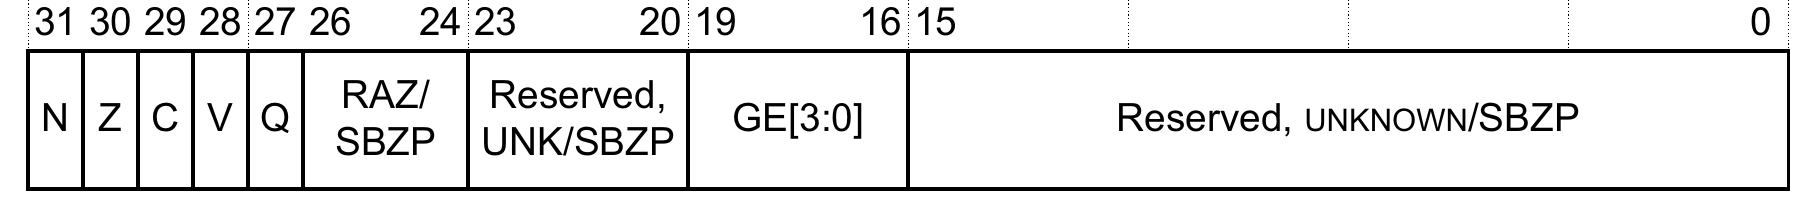
\includegraphics[width=0.6\textwidth]{APSR.png}\\
  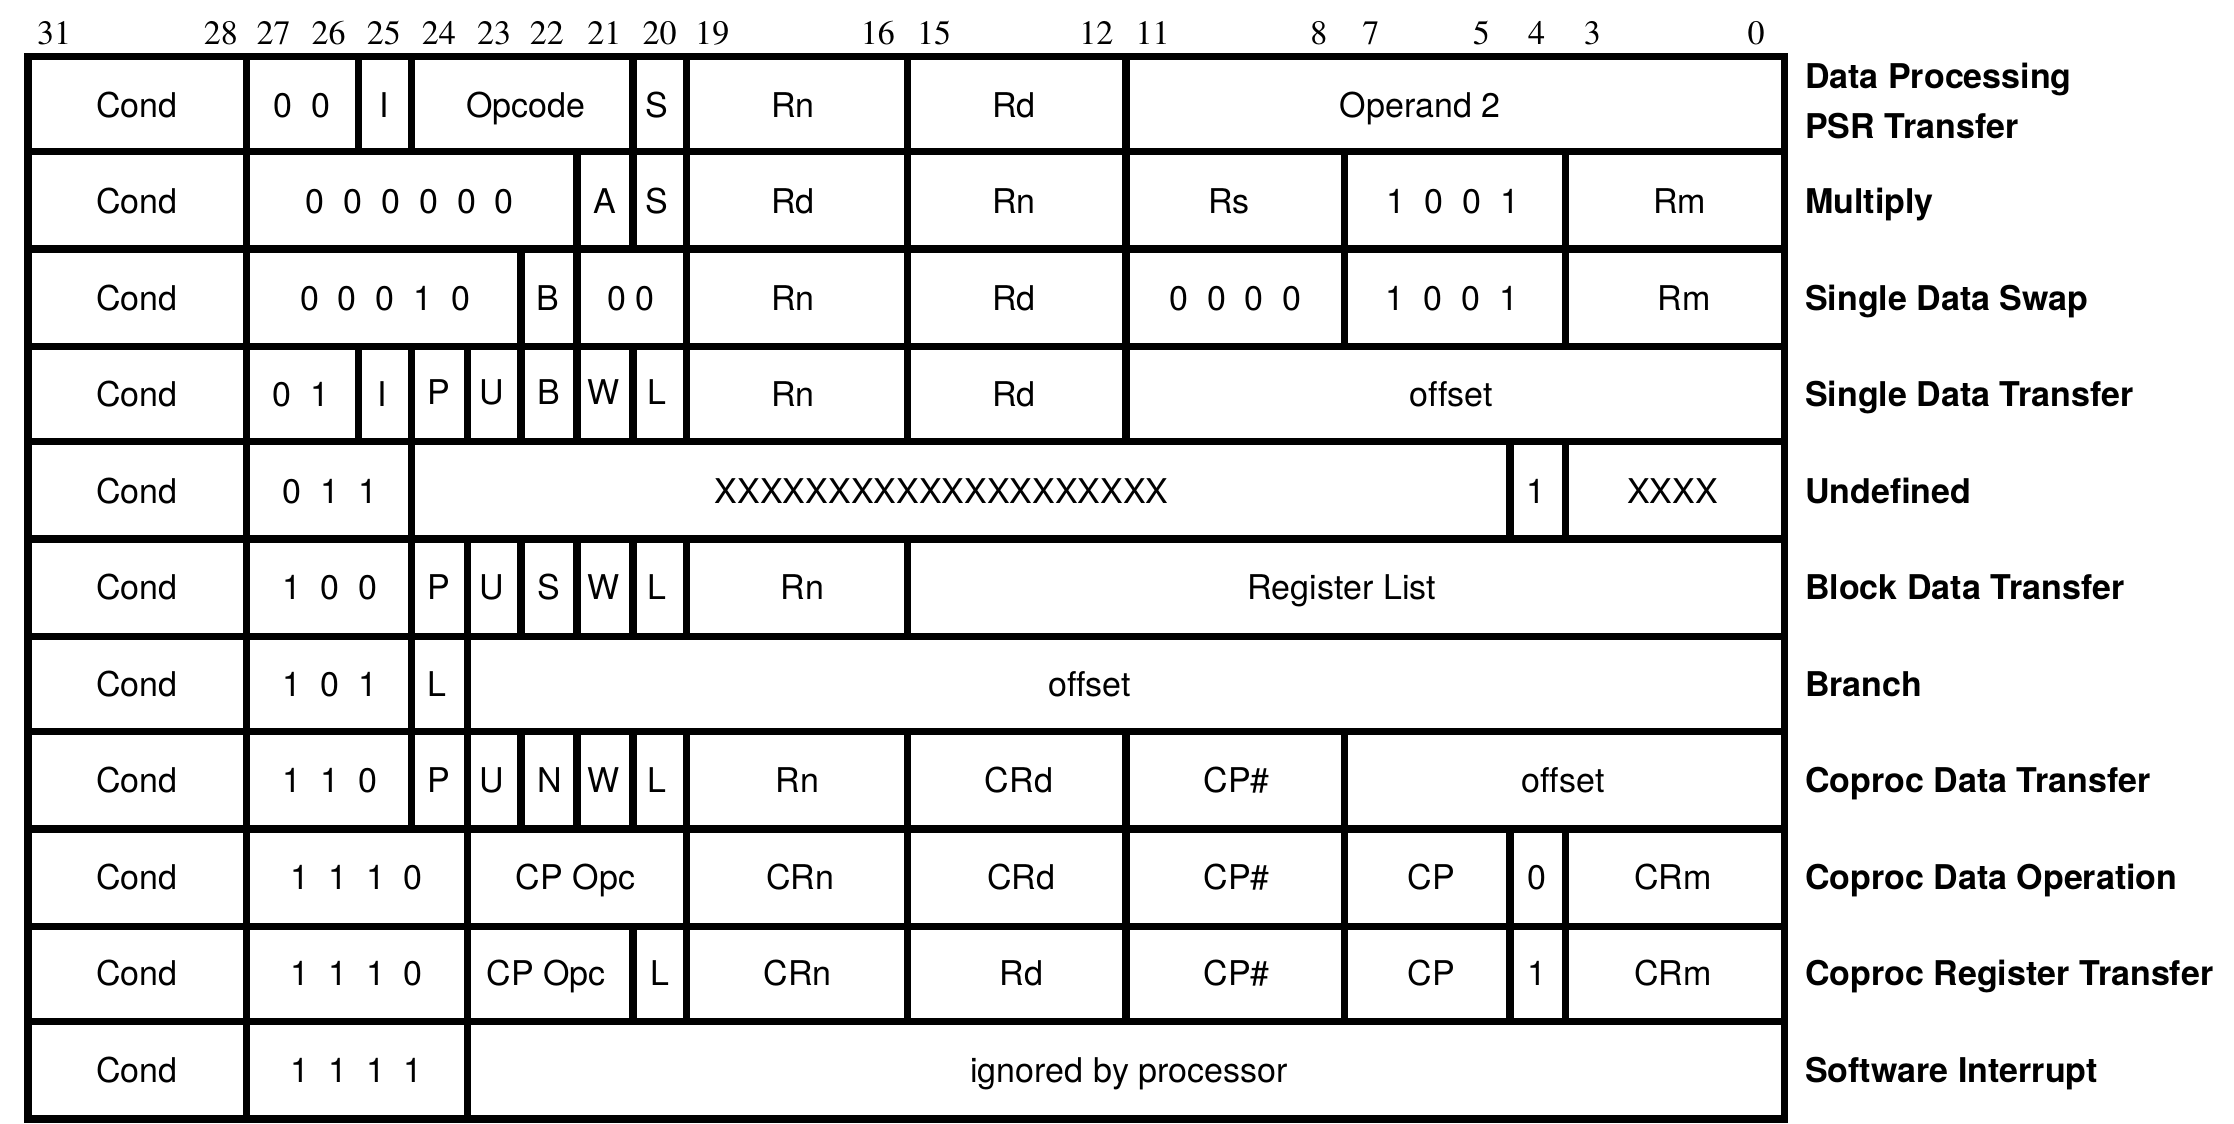
\includegraphics[width=.75\textwidth]{instrucciones.png}}
 \only<2->{
    \tikz[overlay,remember picture]{\draw[rounded corners,top color=red,bottom color=blue,draw=white,thick,fill opacity=0.5] ($(condicion)+(0,0.85)$) rectangle ($(condicion)+(0.085\textwidth,-5.9)$);}
    \begin{textblock}{125}(4,9)
     {\scriptsize{\color{red}Comparación}}
    \end{textblock}   
    \begin{textblock*}{0.3\textwidth}(9.8cm,1.8cm)
     \textbf{CPSR Register}
    \end{textblock*}
  }
\end{frame}

\begin{frame}{Códigos de condición y su significado}
\begin{footnotesize}
\vspace{-0.5cm}
\begin{center}
\begin{tikzpicture}
\node (tbl) { 
 \rowcolors[]{1}{}{gray!5}
 \begin{tabularx}{\textwidth}{p{.18\textwidth} p{.21\textwidth} p{.38\textwidth} p{.15\textwidth} }
 \textbf{\color{white} Mnemónico} & \textbf{\color{white} Flag} & \textbf{\color{white} Significado} & \textbf{ \color{white} Código}\\
  EQ &  Z=1 & Equal & 0000\\
  NE &  Z=0 & Not Equal & 0001\\
  CS/HS &  C=1 & $\geq$ No Signado  & 0010\\
  CC/LO &  C=0 & $<$ No Signado& 0011 \\
  MI &  N=1 & Negativo & 0100 \\
  PL &  N=0 & Positivo o Cero & 0101\\
  VS &  V=1 & Overflow & 0110\\
  VC &  V=0 & No Overflow & 0111\\
  HI &  C=1, Z=0 & $>$ No Signado & 1000\\
  LS &  C=0, Z=1 & $\leq$ No Signado & 1001\\
  GE &  $N \geq V$ & $\geq$ Signado & 1010\\
  LT &  $N \neq V$ & $<$Signado & 1011\\
  GT &  Z=0, N=V & $>$Signado & 1100\\
  LE &  Z=1, $N \neq V$ & $\leq$Signado & 1101\\
  AL & Siempre & Default & 1110\\
\end{tabularx}
};
\begin{pgfonlayer}{background}
\draw[rounded corners,top color=red,bottom color=black,draw=white] ($(tbl.north west)+(0.14,0)$) rectangle ($(tbl.north east)-(0.13,0.45)$);
\draw[rounded corners,top color=white,bottom color=black, middle color=red,draw=blue!20] ($(tbl.south west)+(0.12,0.5)$) rectangle ($(tbl.south east)-(0.12,0)$);
\draw[top color=blue!1,bottom color=blue!20,draw=white] ($(tbl.north east)-(0.13,0.6)$) rectangle ($(tbl.south west)+(0.13,0.2)$);
\end{pgfonlayer}
\end{tikzpicture}
\end{center}
\end{footnotesize}
\end{frame}

\begin{frame}[fragile]{Ejemplo en Modo \arm. Máximo Común Divisor}
 \begin{textblock*}{\textwidth}(0.3cm,1.0cm)
  \begin{block}{Algoritmo de Euclides}
   \lstset{language=[ansi]C,}
   \begin{lstlisting}[escapechar=\@,]
while (a != b) {  /*a y b son los dos n@\color{purple}\'u@meros*/
	 if (a > b) a = a - b;
	 else b = b - a;
}
   \end{lstlisting}
  \end{block}
 \end{textblock*}
 \begin{textblock*}{.48\textwidth}(0.3cm,4.1cm)
  \begin{onlyenv}<2->
   \begin{block}{Con saltos}
    \lstset{language=[ARM]Assembler, basicstyle=\scriptsize,}
    \begin{lstlisting}[escapechar=\@,]
gcd: CMP r0,r1    ;a > b?
     BEQ end      ;a=b? termina
     BLT less     ;a < b salta
     SUB r0,r0,r1 ;a = a-b
     B gcd        ;otro loop
less:SUB r1,r1,r0 ;b = b-a
     B gcd
end:
    \end{lstlisting}
   \end{block}
  \end{onlyenv}
 \end{textblock*}
 \begin{textblock*}{.48\textwidth}(8.3cm,4.1cm)
  \begin{onlyenv}<3->
   \begin{block}{Ejecución Condicional}
    \begin{lstlisting}[escapechar=\@,]
gcd:    CMP   r0, r1
        SUBGT r0, r0, r1
        SUBLT r1, r1, r0
        BNE gcd
    \end{lstlisting}
   \end{block}
  \end{onlyenv}
 \end{textblock*}
\end{frame}

\begin{frame}[t]{Análisis temporal}
  \begin{textblock*}{\textwidth}(.3cm,1.2cm) 
    \begin{itemize}[<+(1)->] \justifying \parskip .2cm
  \item La eficiencia de la ejecución condicional respecto de la compresión de código es evidente: 7 instrucciones (\SI{28}{\byte}) se reducen a 4 tan solo instrucciones (\SI{16}{\byte}).
  \item Esto Resulta en una compresión del código de 43 \% aproximadamente.
  \item Nos proponemos analizar la eficiencia de la ejecución condicional en términos de su impacto en el pipeline
  \item Para ello es necesario recordar que las instrucciones de ARM se ejecutan en 1 ciclo de clock, con excepciones.
 \end{itemize}
\end{textblock*}
\end{frame}
  
\begin{frame}{Análisis temporal}
 \begin{textblock*}{\textwidth}(.3cm,1.2cm) 
  \begin{itemize}[<+(1)->] \justifying \parskip .2cm
   \item Los branches son una de esas excepciones. Tienen dos situaciones posibles:
   \begin{itemize} \justifying \parskip .2cm
    \item {\color{blue}[-] \textbf{Branch No Taken}} No salta por lo tanto continúa con la instrucción siguiente al branch, a la que denominamos \textit{\color{blue}sucesora secuencial}. 
    \item {\color{blue}[-] \textbf{Branch Taken}} Se rompe la secuencia de OPCODE FETCH. El PC cambia a la instrucción \textit{\color {blue}Target} (se denomina así a la instrucción destino del salto). Se vacía el pipeline ya que las instrucciones que contiene corresponden a las \textit{\color{blue}sucesoras secuenciales}.
   \end{itemize}
   \item Un \textbf{\color{blue}Branch No Taken} toma 1 ciclo de clock y no ejecuta (no consume recursos de la CPU). 
   \item Un \textbf{\color{blue}Branch Taken} consume 3 ciclos de clock (uno por cada etapa del pipeline que debe volver a llenarse). 
  \end{itemize}
 \end{textblock*}
\end{frame}

\begin{frame}[fragile]{Análisis temporal}
 \begin{textblock*}{.77\textwidth}(.3cm,1.2cm) 
  \begin{footnotesize}
   \begin{tikzpicture}
    \node (tbl) {
     \rowcolors[]{1}{}{gray!5}
     \begin{tabularx}{\textwidth}{c c l c }
 \textbf{\color{white} R0:a} & \textbf{\color{white} R1:b} & \textbf{\color{white} Instrucción} & \textbf{ \color{white} Ciclos (ARM7)}\\
  1 &  2 & CMP r0, r1 & 1\\
  1 &  2 & BEQ end & 1 (no-taken)\\
  1 &  2 & BLT less  & 3 (taken)\\
  1 &  2 & SUB r1,r1,r0 & 1\\
  1 &  2 & B gcd & 3 (taken)\\
  1 &  1 & CMP r0, r1 & 1\\
  1 &  1 & BEQ end & 3 (taken)\\
    &      &       & \textbf{\color{red}Total: 13}\\
     \end{tabularx}
    };
    \begin{pgfonlayer}{background}
     \draw[rounded corners,top color=blue,bottom color=black,draw=white] ($(tbl.north west)+(0.14,0)$) rectangle ($(tbl.north east)-(4.93,0.45)$);
     \draw[rounded corners,top color=white,bottom color=black, middle color=blue,draw=blue!20] ($(tbl.south west)+(0.12,0.5)$) rectangle ($(tbl.south east)-(4.93,0)$);
     \draw[top color=blue!1,bottom color=blue!20,draw=white] ($(tbl.north east)-(4.93,0.6)$) rectangle ($(tbl.south west)+(0.13,0.2)$);
    \end{pgfonlayer}
   \end{tikzpicture}
  \end{footnotesize}
 \end{textblock*}
 \begin{textblock*}{.45\textwidth}(.6\textwidth,1.2cm)
  {\scriptsize{Usando Branches}}
  \vspace{-0.4cm}
  \begin{lstlisting}[escapechar=\@,]
gcd: CMP r0,r1
     BEQ end
     BLT less
     SUB r0,r0,r1
     B gcd
less:SUB r1,r1,r0
     B gcd
  \end{lstlisting} 
 \end{textblock*}   
 \begin{textblock*}{.77\textwidth}(.3cm,5cm) 
  \begin{scriptsize}
   \begin{tikzpicture}
    \node (tbl1) {
     \rowcolors[]{1}{}{gray!5}
     \begin{tabularx}{\textwidth}{c c l c }
 \textbf{\color{white} R0:a} & \textbf{\color{white} R1:b} & \textbf{\color{white} Instrucción} & \textbf{ \color{white} Ciclos (ARM7)}\\
  1 &  2 & CMP r0, r1 & 1\\
  1 &  2 & SUBGT r0,r0,r1 & 1(no ejecutada)\\
  1 &  1 & SUBLT r1,r1,r0 & 1\\
  1 &  1 & BNE gcd & 3 (taken)\\
  1 &  1 & CMP r0, r1 & 1\\
  1 &  1 & SUBGT r0,r0,r1 & 1 (no ejecutada)\\
  1 &  1 & SUBLT r1,r1,r0 & 1 (no ejecutada)\\
  1 &  1 & BNE gcd & 1 (no taken)\\
    &      &       & \textbf{\color{red}Total: 10}\\
    & & & \\
     \end{tabularx}
    };
    \begin{pgfonlayer}{background}
     \draw[rounded corners,top color=blue,bottom color=black,draw=white] ($(tbl1.north west)+(0.14,0)$) rectangle ($(tbl1.north east)-(4.93,0.45)$);
     \draw[rounded corners,top color=white,bottom color=black, middle color=blue,draw=blue!20] ($(tbl1.south west)+(0.12,0.5)$) rectangle ($(tbl1.south east)-(4.93,0)$);
     \draw[top color=blue!1,bottom color=blue!20,draw=white] ($(tbl1.north east)-(4.93,0.6)$) rectangle ($(tbl1.south west)+(0.13,0.2)$);
    \end{pgfonlayer}
   \end{tikzpicture}
  \end{scriptsize}
 \end{textblock*} 
 \begin{textblock*}{.45\textwidth}(.6\textwidth,5.2cm)
  {\scriptsize{Ejecución Condicional}}
  \vspace{-0.4cm}
  \begin{lstlisting}[escapechar=\@,]
gcd: CMP   r0, r1
     SUBGT r0, r0, r1
     SUBLT r1, r1, r0
     BNE gcd
  \end{lstlisting}
 \end{textblock*}   
\end{frame}

\begin{frame}{El segundo operando}
 \begin{textblock*}{\textwidth}(.3cm,1.1cm) 
  \begin{itemize}[<+(1)->] \justifying
   \item Puede ser una constante. \textbf{\texttt{\#valor}}.
   \item Puede ser un registro. \textbf{\texttt{Rm}}
   \item El registro puede llevar desplazamiento. \textbf{\texttt{Rm, \{shift\}}} \\
   \texttt{\textbf{shift}} se aplica al registro \textbf{\texttt{Rm}}. Si lo omitimos, se usa \textbf{\texttt{Rm}} sin cambios
   \begin{itemize}\justifying
    \item [-] \textbf{\texttt{\color{blue}ASR \#n}}. \textbf{A}rithmetic \textbf{S}hift \textbf{R}ight, \textbf{\texttt{\#n}} bits, con $1 \leq  n \leq 32$ (si $n \geq 32$, todos los bits del registro quedan con el nit [31] del registro y el Carry mantiene el bit [31])
    \item [-] \textbf{\texttt{\color{blue}LSL \#n}}. \textbf{L}ogical \textbf{S}hift \textbf{L}eft, \textbf{\texttt{\#n}} bits, con $1 \leq  n \leq 31$ (si $n \geq 32$, todos los bits del registro quedan en '0', y el Carry recibe el bit [31], si $n = 33$ el Carry quedará en '0')
    \item [-] \textbf{\texttt{\color{blue}LSR \#n}}. \textbf{L}ogical \textbf{S}hift \textbf{R}ight, \textbf{\texttt{\#n}}    bits, con $1 \leq  n \leq 32$ (si $n=32$, todos los bits del registro quedan en '0', y el Carry recibe el bit [31], si $n =33$ el Carry quedará en '0')
    \item [-] \textbf{\texttt{\color{blue}ROR \#n}}. \textbf{RO}tate \textbf{R}ight, \textbf{\texttt{\#n}} bits, con $1 \leq  n \leq 31$ (si $n = 32$, tel registro igual, y el Carry recibe el bit [31], si $n > 33$ es equivalente a rotar a derecha $n-32$ bits)
    \item [-] \textbf{\texttt{\color{blue}RRX \#n}}. \textbf{R}otate \textbf{R}ight, one bit with e\textbf{X}tend. Rota a través del Carry.
    \item [-] \textbf{\texttt{\color{blue}\textit{type Rs}}}. Controlado por registro: \texttt{\textit{\textbf{type}}} es \textbf{ASR}, \textbf{LSL}, \textbf{LSR}, o \textbf{ROR},y \textbf{\textit{\texttt{Rn}}} es el registro en el que se especifica la cantidad de bits.
    \item [-] \textbf{\texttt{-}}. En este caso no hay desplazamiento (se aplica \textbf{\texttt{LSL \#0}}).
   \end{itemize}
  \end{itemize}
 \end{textblock*}   
\end{frame}

\begin{frame}{Operaciones de shift}
 \begin{textblock*}{.35\textwidth}(.3cm,1.2cm)
  \only<1->{\flushright 
   Arithmetic Shift Right: ASR \#3}
  \only<2->{\vskip .64cm 
   Logical Shift Right: LSR \#3}
  \only<3->{\vskip .72cm
   Logical Shift Left: LSL \#3}
  \only<4->{\vskip .9cm
   Rotate Right:  ROR \#3}
  \only<5->{\vskip .75cm
   Rotate Right with eXtend}
 \end{textblock*}
 \begin{textblock*}{.5\textwidth}(.4\textwidth,1.2cm)
  \only<1->{\centering 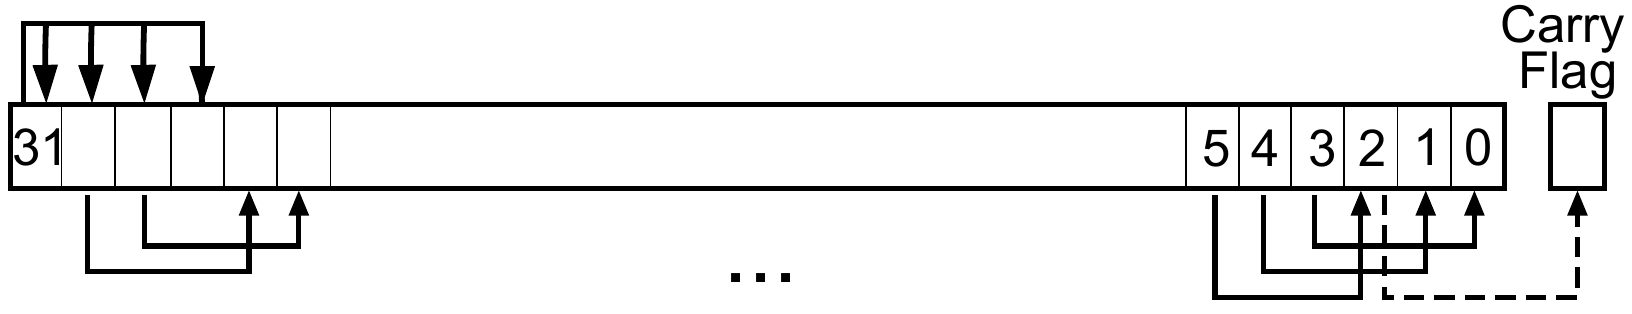
\includegraphics[width=.9\textwidth]{ASR-3.png}\\}
  \only<2->{\centering 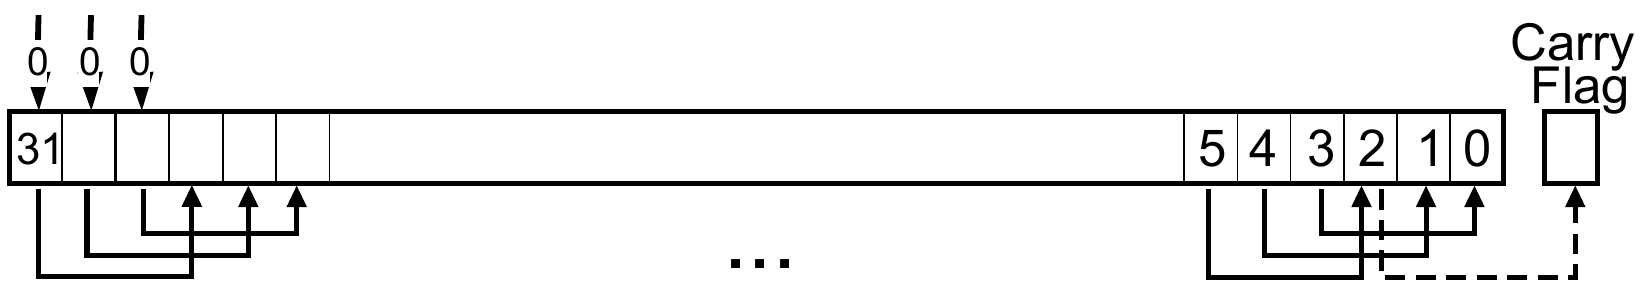
\includegraphics[width=.9\textwidth]{LSR-3.png}\\}
  \only<3->{\centering 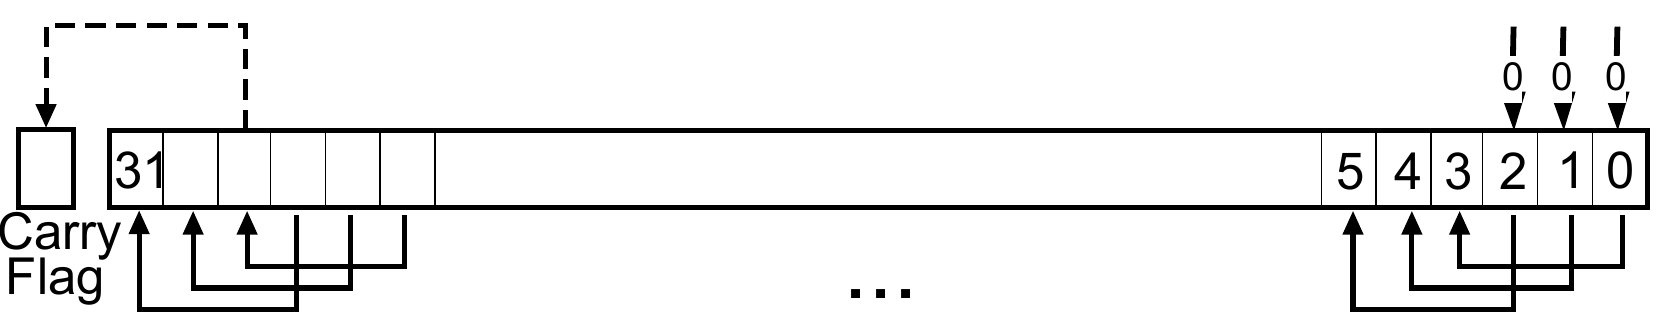
\includegraphics[width=.9\textwidth]{LSL-3.png}\\}
  \only<4->{\centering 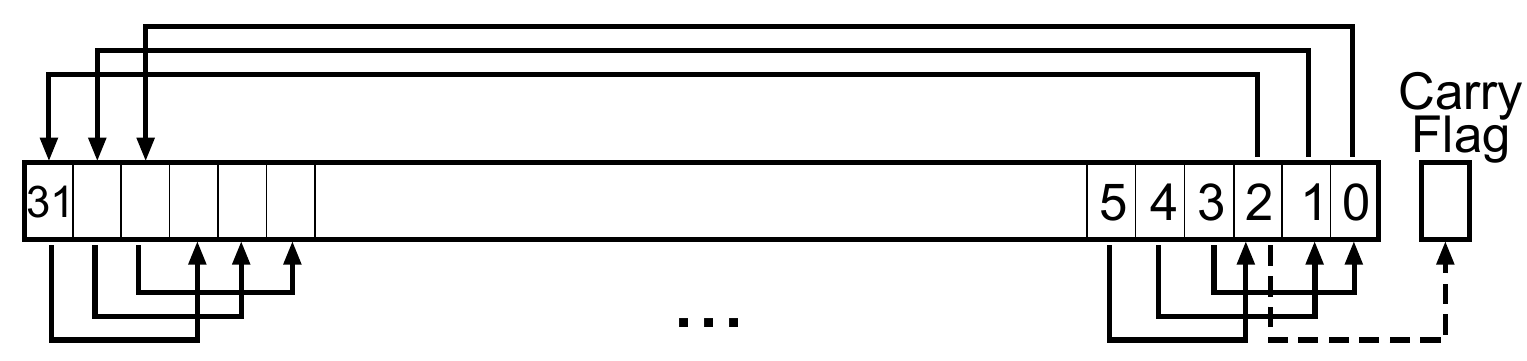
\includegraphics[width=.9\textwidth]{ROR-3.png}\\}
  \only<5->{\centering 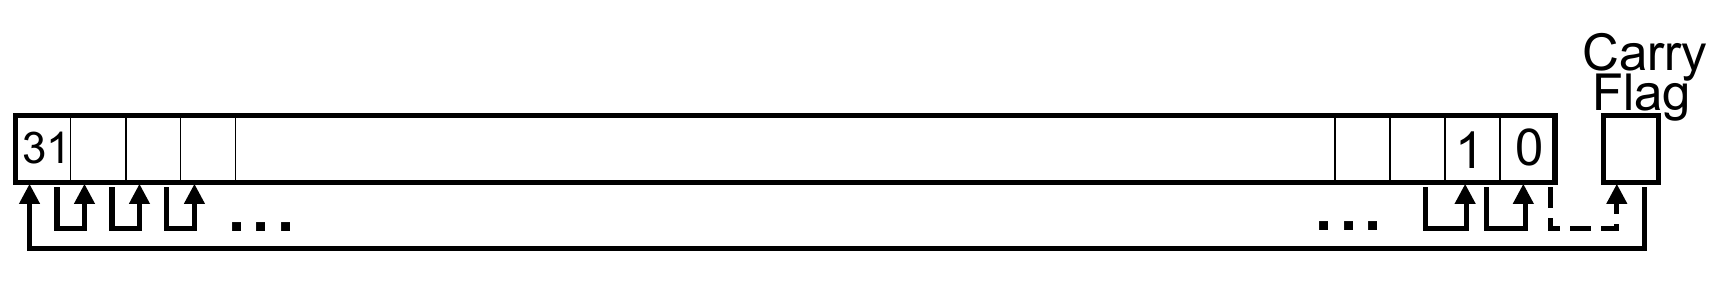
\includegraphics[width=.9\textwidth]{RRX.png}\\}
 \end{textblock*}
\end{frame}

\subsection{Acceso a memoria Load - Store}
\begin{frame}{Lectura: Load}
 \begin{textblock*}{\textwidth}(.3cm,1.2cm)
  \begin{itemize}[<+->]\parskip .3cm
   \item Lectura simple
   \begin{itemize}\parskip .3cm
    \item Direccionamiento Inmediato
    \item Direccionamiento Relativo a Program Counter (R15)
    \item Direccionamiento con Offset en Registro
   \end{itemize}
   \item Lectura Múltiple
  \end{itemize}
 \end{textblock*}
\end{frame}

\begin{frame}[fragile]{Load con Desplazamiento Inmediato}
 \begin{textblock*}{\textwidth}(.3cm,1.2cm)
  \textbf{Sintaxis}
 \end{textblock*}
 \footnotesize
\begin{textblock*}{\textwidth}(.3cm,1.8cm)
\ttfamily \obeyspaces
\uncover<1->{\textcolor{blue}{LDR\{type\}\{cond\}} Rt, [Rn \{, \#offset\}] \textcolor{purple}{; immediate offset}.}\\
\uncover<2->{\textcolor{blue}{LDR\{type\}\{cond\}} Rt, [Rn, \#offset]!   \textcolor{purple}{; pre-indexed.}}\\
\uncover<3->{\textcolor{blue}{LDR\{type\}\{cond\}} Rt, [Rn], \#offset    \textcolor{purple}{; post-indexed.}}\\
\uncover<4->{\textcolor{blue}{LDRD\{cond\}} Rt, Rt2, [Rn \{, \#offset\}] \textcolor{purple}{; immediate offset, doubleword.}}\\
\uncover<5->{\textcolor{blue}{LDRD\{cond\}} Rt, Rt2, [Rn, \#offset]!   \textcolor{purple}{; pre-indexed, doubleword.}}\\
\uncover<6->{\textcolor{blue}{LDRD\{cond\}} Rt, Rt2, [Rn], \#offset    \textcolor{purple}{; post-indexed, doubleword.}}\\
\end{textblock*}
 \begin{textblock*}{\textwidth}(.3cm,4.5cm)
  \begin{itemize}
   \item<7-> [] \textit{\texttt{type}}: \textbf{B} unsigned Byte, \textbf{H} unsigned Half-word, \textbf{SB} Signed Byte, \textbf{SH} Signed Half-word, \textbf{-} Word
   \item<8-> [] \texttt{\textit{cond}}:     \textbf{Código de Condición (opcional)}
   \item<9-> [] \texttt{\textit{Rt}}:       \textbf{Registro a cargar (operando destino)}
   \item<10-> [] \textit{\texttt{Rn}}:       \textbf{Registro puntero a memoria.}
   \item<11-> [] \textit{\texttt{\#offset}}: \textbf{Offset (optativo). Si se incluye se suma a \texttt{\textit{R}n}}
   \item<12-> [] \texttt{\textit{Rt2}}:      \textbf{Si la operación es de doble word, este registro carga la word alta.}
  \end{itemize}
 \end{textblock*}
\end{frame}

\begin{frame}[fragile]{Ejemplos}
 \begin{textblock*}{\textwidth}(.3cm,.9cm)%\color{gray97}\pgfsetfillopacity{1},]
  \begin{lstlisting}[escapechar=\@, basicstyle=\scriptsize, backgroundcolor=, ] 
LDR    r8,[r10]     ;carga R8 desde la direcci@\color{purple}\'o@n apuntada por R10.
LDRNE  r2,[r5,#960]!;Carga R2 condicionalmente desde la direcci@\color{purple}\'o@n 
                    ;apuntada por (R5+960), e incrementa R5 en 960.
;Indexaci@\color{purple}\'o@n = Autoincremento. Tres casos:
LDR    r0,[r4, #4]  ;offset simple: R0 = *(int*)(R4+4); R4 no cambia
LDR    r0,[r4, #4]! ;pre-indexed:   R0 = *(int*)(R4+4); R4 = R4+4
LDR    r0,[r4], #4  ;post-indexed:  R0 = *(int*)(R4+0); R4 = R4+4
;Indexdo con desplazamiento
LDR    r9,[r10, r2, LSL #4] ;r9 = *(int*) (r10 + (r2 << 4) )
;Lectura de Doble word -> Solo disponible en Modo ARM
LDRD   r6,r7,[r10]  ; r7 = *(int*)(r10) y r6 = *(int*)(r10+4)
; es equivalente a esta secuencia
LDR    r6,[r10]
LDR    r7,[r10, #4]
;N@\color{purple}\'u@meros signados
LDRSH  r5,[r0]      ; Valores iniciales r0 = 0x5F006EC0, r5 0x12345678
                    ; Memoria:  0x5F006EC0  0xFA---
                    ;           0x5F006EC1  0x91---|---
                    ;           0x5F006EC2  0x23   |   |
                    ;           0x5F006EC3  0xA5   |   |
                    ; Resultado r5 = 0xFFFF91FA<---    |
                    ;                      ^-----------                                            
  \end{lstlisting}
 \end{textblock*}
\end{frame}

\begin{frame}[fragile]{Load Relativo al Program Counter}
\footnotesize
 \begin{textblock*}{\textwidth}(.3cm,1.2cm)
 \textbf{Sintaxis}
 \end{textblock*}
 \begin{textblock*}{\textwidth}(.3cm,1.5cm)
  \ttfamily \obeyspaces
  \uncover<1->{\textcolor{blue}{LDR\{type\}\{cond\}\{.W\}}  Rt, label}\\
  \uncover<2->{\textcolor{blue}{LDRD\{cond\}}           Rt, Rt2, label \textcolor{purple}{; Doubleword.}}\\
 \end{textblock*}
 \begin{textblock*}{\textwidth}(0cm,2.2cm)
  \begin{itemize}
   \item<3-> []\textit{\texttt{type}}: \textbf{B} unsigned Byte, \textbf{H} unsigned Half-word, \textbf{SB} Signed Byte, \textbf{SH} Signed Half-word, \textbf{-} Word
   \item<4-> [] \texttt{\textit{cond}}:  Código de Condición (opcional)
   \item<5-> [] \texttt{\textit{Rt}}:    Registro a cargar (operando destino)
   \item<6-> [] \textit{\texttt{.W}}:    Especificador de ancho de instrucción (Solo \Thdos).
   \item<7-> [] \textit{\texttt{Label}}: El el número a sumar al PC (en Ca2)
   \item<8-> [] \texttt{\textit{Rt2}}:   Si la operación es de doble word, este registro carga la word alta.
  \end{itemize}
 \end{textblock*}
 \begin{textblock*}{\textwidth}(.3cm,5.2cm)
  \begin{itemize}
   \item<9-> [] Ejemplo:
   \end{itemize}
  \end{textblock*}
  \begin{textblock*}{\textwidth}(.3cm,5.6cm)
   \begin{onlyenv}<9->
    \begin{lstlisting}[escapechar=\@, basicstyle=\scriptsize, backgroundcolor=,]
.section .text
.global _start
_start:
   ldr r0, =jump        /* load the address of the function label jump into R0 */
   ....
jump:
   ldr r2, =511         /* load the value 511 into R2 */ 
   bkpt
   \end{lstlisting}
  \end{onlyenv}
 \end{textblock*}
\end{frame}

\begin{frame}[fragile]{Load con Desplazamiento en Registro}
 \footnotesize
 \begin{textblock*}{\textwidth}(.3cm,1.2cm)
 \textbf{Sintaxis}
 \end{textblock*}
 \begin{textblock*}{\textwidth}(.3cm,1.4cm)
  \ttfamily \obeyspaces
  \uncover<1->{\textcolor{blue}{LDR\{type\}\{cond\}} Rt, [Rn,$\pm$ Rm {shift}]    \textcolor{purple}{; offset registro}.}\\
  \uncover<2->{\textcolor{blue}{LDR\{type\}\{cond\}} Rt, [Rn,$\pm$ Rm {shift}]!   \textcolor{purple}{; pre-indexed (A32).}}\\
  \uncover<3->{\textcolor{blue}{LDR\{type\}\{cond\}} Rt, [Rn],$\pm$ Rm {shift}    \textcolor{purple}{; post-indexed (A32).}}\\
  \uncover<4->{\textcolor{blue}{LDRD\{cond\}} Rt, Rt2, [Rn,$\pm$ Rm]          \textcolor{purple}{; offset registro, dword (A32).}}\\
  \uncover<5->{\textcolor{blue}{LDRD\{cond\}} Rt, Rt2, [Rn,$\pm$ Rm]!         \textcolor{purple}{; pre-indexed, doubleword (A32).}}\\
  \uncover<6->{\textcolor{blue}{LDRD\{cond\}} Rt, Rt2, [Rn],$\pm$ Rm          \textcolor{purple}{; post-indexed, doubleword (A32).}}\\%C
 \end{textblock*}
 \begin{textblock*}{\textwidth}(.3cm,3.6cm)
  \begin{itemize}
   \item<7-> []\textit{\texttt{type}}: \textbf{B} unsigned Byte, \textbf{H} unsigned Half-word, \textbf{SB} Signed Byte, \textbf{SH} Signed Half-word, \textbf{-} Word
   \item<8-> [] \texttt{\textit{cond}}: Código de Condición (opcional)
   \item<9-> [] \texttt{\textit{Rt}}:   Registro a cargar (operando destino)
   \item<10-> [] \textit{\texttt{Rn}}:   Registro puntero a memoria.
   \item<11-> [] \textit{\texttt{Rm}}:   Registro que contiene el Offset. No permitido en T32
   \item<12-> [] \texttt{\textit{Rt2}}:  Si la operación es de doble word, este registro carga la word alta.
  \end{itemize}
 \end{textblock*}
 \begin{textblock*}{\textwidth}(.3cm,7cm)
  \only<13->{\textbf{Ejemplos:}}
 \end{textblock*}
 \begin{textblock*}{\textwidth}(.3cm,7.2cm)
  \begin{onlyenv}<13->
   \begin{lstlisting}[escapechar=\@, basicstyle=\scriptsize, backgroundcolor=,]
LDR  r1,[r0,r3]    ;Carga r1 con la word apuntada por r0+r3
LDRD r1,r2 [r0,r3] ;Igual que el caso anterior pero lee dword
LDR  r1,[r0],r3    ;Primer caso pero con post-incremento.
   \end{lstlisting}
  \end{onlyenv}
 \end{textblock*}
\end{frame}

\begin{frame}[fragile]{Load Multiple}
 \begin{textblock*}{\textwidth}(.3cm,0.9cm)
  \begin{itemize}
   \item Sintaxis
  \end{itemize}
 \end{textblock*}
 \begin{footnotesize}
  \begin{textblock*}{\textwidth}(.3cm,1.2cm)
    \begin{onlyenv}<1->
    \begin{verbatim}
LDM{addr_mode}{cond} Rn{!}, reglist{^}
    \end{verbatim}
   \end{onlyenv}
  \end{textblock*}
  \begin{textblock*}{\textwidth}(.3cm,1.8cm)
   \begin{itemize}[<+(1)->]
    \item [] \textit{\texttt{addr\_mode}}: Tratamiento de \textit{\texttt{Rn}}: \textbf{IA} Increment After, \textbf{IB} Increment Before, \textbf{DA} Decrement After, \textbf{DB} Decrement Before.
    \item [] \texttt{\textit{cond}}: Código de Condición (opcional)
    \item [] \textit{\texttt{Rn}}: Registro puntero Base a memoria.
    \item [] \texttt{\textit{!}}: Escribe dirección final en \textit{\texttt{Rn}}
    \item [] \textit{\texttt{reglist}}: Lista de registros destino. Puede contener rangos
   \end{itemize}
  \end{textblock*}
  \begin{textblock*}{\textwidth}(.3cm,4.8cm)
   \begin{itemize}[<+(1)->]
    \item Ejemplos:
   \end{itemize}
  \end{textblock*}
  \begin{textblock*}{\textwidth}(.3cm,5.2cm)
   \begin{onlyenv}<7->
    \begin{lstlisting}[escapechar=\@, basicstyle=\scriptsize, backgroundcolor=,]
LDMIA r7,{r0-r3,r8,r12} ;Carga r0 a r3, r8 y r9, con las seis words
                        ;almacenadas a partir de la direcci@\color{purple}\'o@n 
                        ;apuntada por r7
    \end{lstlisting}
   \end{onlyenv}
  \end{textblock*}
  \begin{textblock*}{\textwidth}(.3cm,6.5cm)
   \begin{onlyenv}<8->
    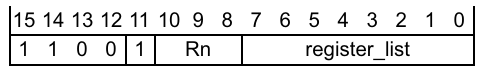
\includegraphics[width=.34\textwidth]{InstFormatLDMT.png}
    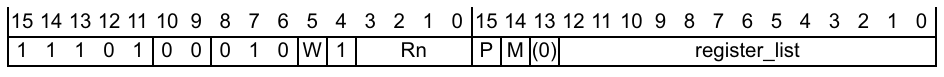
\includegraphics[width=.62\textwidth]{InstFormatLDMT2.png}\\
    Modo \Thumb: \SI{8}{\bit} [R7-R0] \hfill Modo Tumb-2 PC,LR,[R12-R0]
   \end{onlyenv}
   \begin{onlyenv}<9->
    \centering 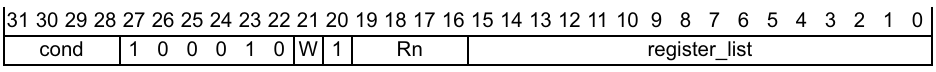
\includegraphics[width=.7\textwidth]{InstFormatLDMArm.png} Modo \arm{}32 [R15-R0]\\
   \end{onlyenv}
  \end{textblock*}
\end{footnotesize} 
\end{frame}

\begin{frame}[fragile]{Escrituras: Store}
 \begin{textblock*}{\textwidth}(.3cm,.9cm)
  \begin{itemize}[<+(1)->] \justifying
   \item La sintaxis es la misma, a excepción del Mnemónico, que en este caso es STR, STRD (para dobles word)
   \item Modos de direccionamiento: Offset inmediato, y Offset Registro.
   \item Para bytes y hwords no extiende signo (tamaño destino idéntico).
   \item Ejemplos:
  \end{itemize}
 \end{textblock*}
 \begin{textblock*}{\textwidth}(3.3cm,3.1cm)
  \begin{onlyenv}<5->
   \begin{lstlisting}[escapechar=\@, basicstyle=\scriptsize, backgroundcolor=,]
STR    r8,[r10]     ;Escribe R8 en la direcci@\color{purple}\'o@n apuntada por R10.
STRNE  r2,[r5,#960]!;Escribe R2 condicionalmente en la direcci@\color{purple}\'o@n 
                    ;apuntada por (R5+960), e incrementa R5 en 960.
;Indexaci@\color{purple}\'o@n = Autoincremento. Tres casos:
STR    r0,[r4, #4]  ;offset simple: *(int*)(R4+4) = R0; R4 no cambia
STR    r0,[r4, #4]! ;pre-indexed:   *(int*)(R4+4) = R0; R4 = R4+4
STR    r0,[r4], #4  ;post-indexed:  *(int*)(R4+0) = R0; R4 = R4+4
;Indexdo con desplazamiento
STR    r9,[r10, r2, LSL #4] ;*(int*) (r10 + (r2 << 4) ) = r9
;Lectura de Doble word -> Solo disponible en Modo ARM
STRD   r6,r7,[r10]  ; *(int*)(r10) = r7 y *(int*)(r10+4) = r6
; es equivalente a esta secuencia
STR    r6,[r10]
STR    r7,[r10, #4]
STMIA  r5,{r0-r3}   ; Al igual que para LDM, IA es el default      
   \end{lstlisting}
  \end{onlyenv}
 \end{textblock*}
\end{frame}

\subsection{Constantes y literal pools}
\begin{frame}[fragile,plain]
  \Cshadowbox[white!10!black]{blue!80!black}{\justifying
   \justifying
   \textit{``One of the best things about learning assembly language is that you deal directly with hardware, and as a result, learn about computer architecture in a very direct way''.}\\
   \vspace*{0.3cm}
   \hfill ARM Assembly Language\\
   \hfill William Hohl, Christopher Hinds.
  }
   % \end{tcolorbox}
\end{frame}

\begin{frame}[fragile]{Rango de Direccionamiento}
 \begin{textblock*}{\textwidth}(.3cm,1.2cm)
  \begin{itemize}[<+(1)->]
   \justifying
   \item ARM al igual que otras arquitecturas tiene tamaño de instrucciones fijo en \SI{32}{\bit}.
   \item Sin embargo muchas veces se necesita trabajar con operandos inmediatos de \SI{32}{\bit}. Por ejemplo una dirección de memoria.
   \item En particular la arquitectura ARM mapea en memoria todos los dispositivos de E/S, de modo que cuando se los quiera acceder hay que escribir su dirección en un registro del core para utilizarlo como puntero.
   \item Por ejemplo, en un Zynq7000 (Dual Cortex A9), los diferentes periféricos se despliegan a partir de la dirección de memoria 0xE0000000.
   \item ¿Como es posible almacenar esta dirección en un registro del core para utilizarlo como puntero base?.
   \item La instrucción que se requiere es del tipo:
  \end{itemize}
 \end{textblock*}
 \begin{textblock*}{\textwidth}(.3cm,7.2cm)
  \begin{onlyenv}<7->
   \begin{lstlisting}
    MOV r6,#0xE0000000
   \end{lstlisting}
  \end{onlyenv}
 \end{textblock*}
\end{frame}

\begin{frame}{Usando constantes de \SI{32}{\bit}}
 \begin{textblock*}{\textwidth}(.3cm,1.2cm)
  \begin{itemize}
   \item ¿Como es el formato de la instrucción \texttt{MOV}?
  \end{itemize}
 \end{textblock*}
 \begin{textblock*}{\textwidth}(.3cm,2.0cm)
  \only<2->
   { 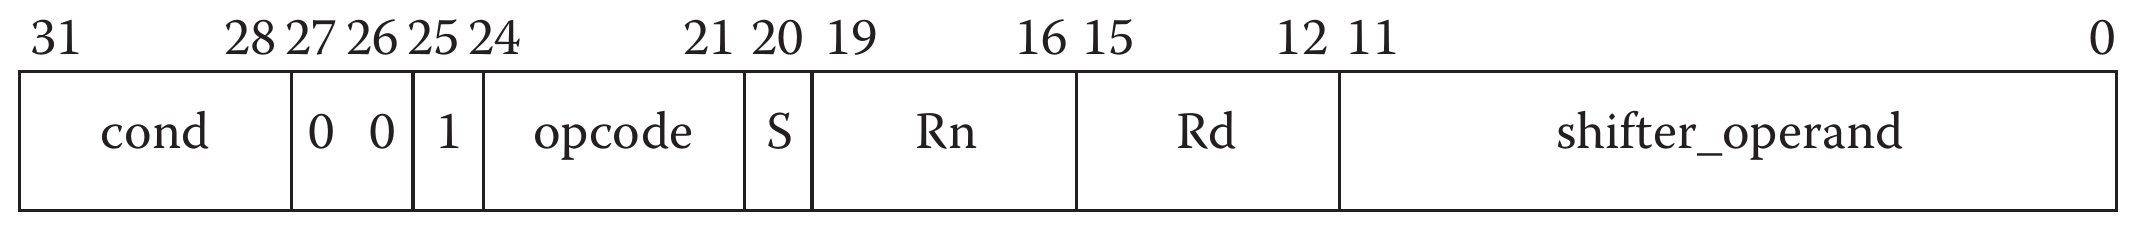
\includegraphics[width=\textwidth]{OpcodeMOV.png}\\
     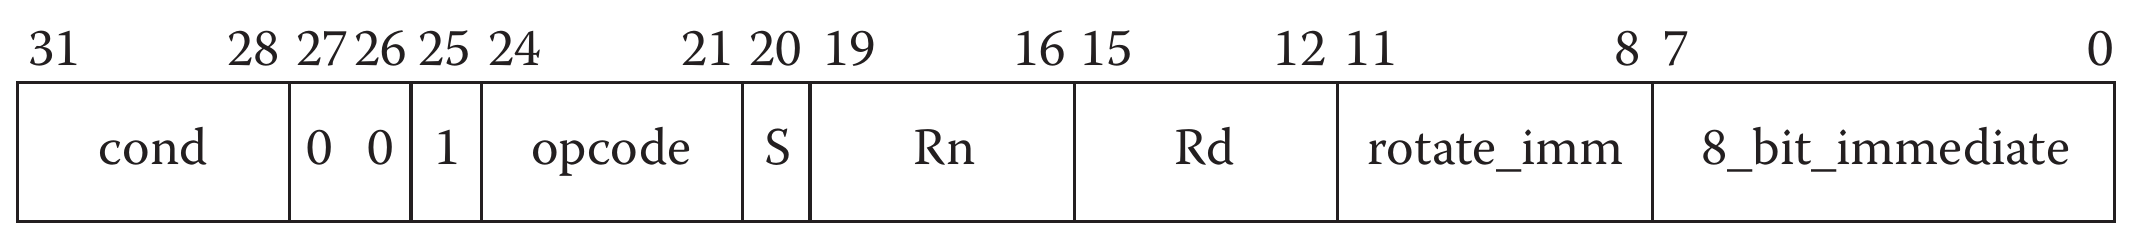
\includegraphics[width=\textwidth]{OpcodeMOVi.png}
     }
 \end{textblock*}
 \begin{textblock*}{\textwidth}(.3cm,5.4cm)
  \begin{itemize}[<+(2)->]
   \item \texttt{MOV} tiene dos opciones:
   \begin{itemize}
    \justifying
    \item [\checkmark] la primera recibe un offset de\SI{12}{\bit} relativo al \textit{Program Counter} que se toma en Ca2 y permite referenciar direcciones entre $\pm$ 4Kbytes.
    \item [\checkmark]La segunda divide el campo de\SI{12}{\bit} en dos: en los 8 LSB un offset, y en los 4 MSB un valor que se multiplica por 2 y permite rotar a la derecha al offset en esa cantidad de bits, a través de un registro temporario interno de \SI{32}{\bit}.
   \end{itemize}
  \end{itemize}
 \end{textblock*}
\end{frame}

\begin{frame}[fragile]{El esquema de rotación}
 \begin{textblock*}{\textwidth}(.3cm,1.2cm)
  \centering 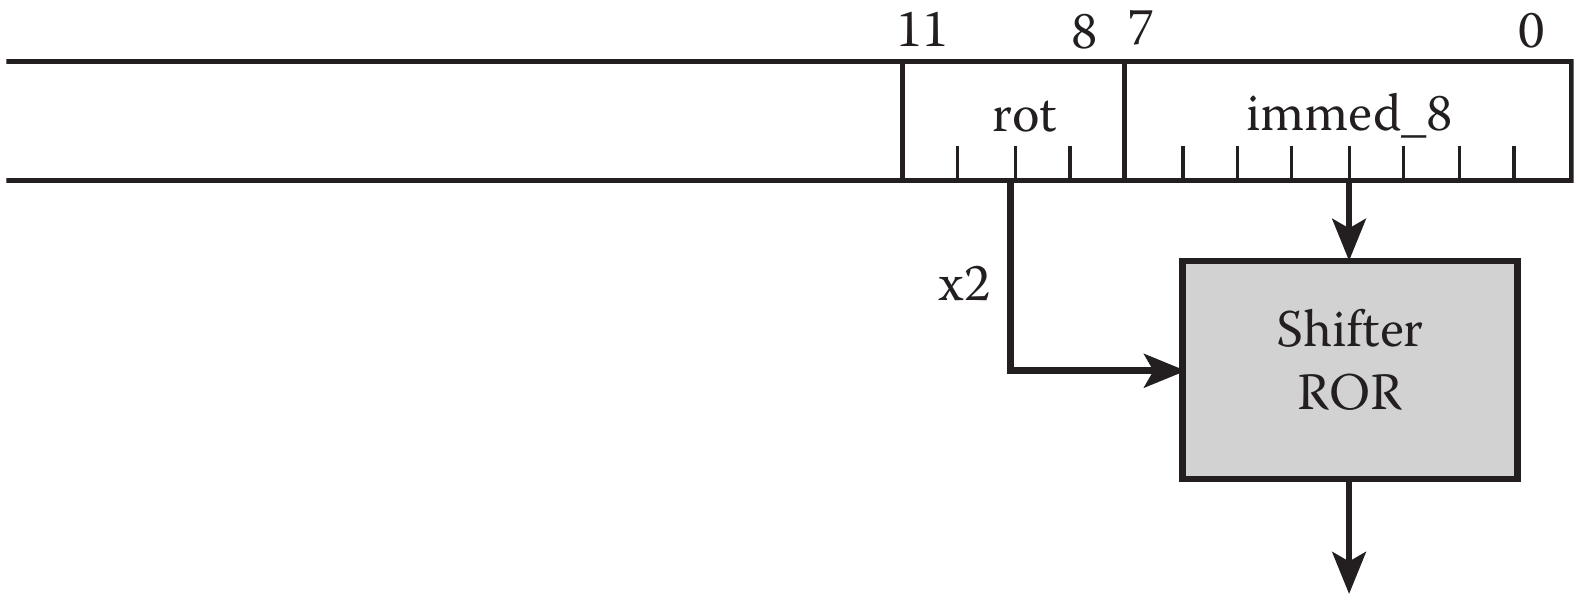
\includegraphics[width=\textwidth]{shifter.png}
 \end{textblock*}
 \begin{textblock*}{0.56\textwidth}(0.5cm,3.2cm)\justifying
  \only<1->{Esto significa que si el bit pattern fuese por ejemplo 0xE3A004FF, el código que se genera es:} 
  \begin{onlyenv}
   \begin{lstlisting}[escapechar=\@, basicstyle=\scriptsize]
mov   r0, #0xFF, 8  ;r0 = 0xFF000000
   \end{lstlisting}
  \end{onlyenv}
  \only<2->{Lo que significa rotar 0xFF 8 lugares a la derecha\\}
  \only<3->{Este funcionamiento es consecuencia de haber incluido en el datapath un barrel shifter en el camino de los operandos de la ALU}
 \end{textblock*}
\end{frame}

\begin{frame}{Estudios previos}
 \begin{textblock*}{\textwidth}(.3cm,1.2cm)
  \begin{itemize}[<+(1)->] \justifying \parskip 0.3cm
   \item La idea es generar \textit{Clases de números} en lugar del rango de valores posibles con \SI{32}{\bit}: 0 a $2^{32}-1$.
   \item Como cada vez que no alcanza el recurso de hardware, observar como funciona el software puede ayudar a encontrar la solución.
   \item ``Mediciones'' (Análisis de código de uso práctico según ARM):
   \begin{itemize} \justifying \parskip 0.3cm
    \item El 50\% de los valores constantes (operandos inmediatos que utilizan los programas de uso práctico) está en el rango [-15,15]
    \item El 90\% está en el rango [-511, 511].
   \end{itemize}
   \item De modo que el approach adoptado para la instrucción \textbf{\texttt{MOV}} parece ser suficiente para resolver una parte significativa del problema, aunque nunca el 100\% de los casos.
  \end{itemize}
 \end{textblock*}
\end{frame}

\begin{frame}[fragile]{Trabajando con Clases de Números}
 \begin{textblock*}{\textwidth}(.3cm,1.2cm)
  \begin{itemize}[<+(1)->] \justifying \parskip 0.2cm
   \item Clases de números: Son conjuntos de números con características similares. Por ejemplo, máscaras de \SI{32}{\bit}.
   \item Una forma de generar otro tipo de máscaras la proporciona la instrucción \texttt{\textbf{MVN}} (Mov Not).\\
   \centering 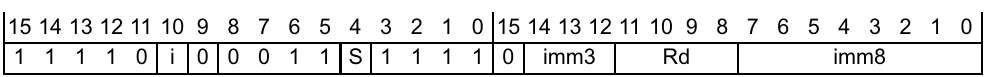
\includegraphics[width=.8\textwidth]{MVN.png}
   \item Es una variante de \textbf{\texttt{MOV}}, que opera de forma idéntica, solo que luego de rotar el número le efectúa la operación NOT (o Ca1).
   \item Ejemplos de clases de máscaras generadas mediante rotación a derecha de un offset de un byte, o con \texttt{\textbf{MVN}}.
  \end{itemize}
 \end{textblock*}
 \begin{textblock*}{.9\textwidth}(1.1cm,6.5cm)
  \begin{onlyenv}<6->
   \begin{lstlisting}[escapechar=\@, basicstyle=\scriptsize]
  mov r6, #0xFF,24   /* OPCODE = E3A06CFF Pone r6 = 0x0000FF00*/
  mov r6, #0x01,30   /* OPCODE = E3A06F01 Pone r6 = 0x00000004*/
  mov r6, #0x01,26   /* OPCODE = E3A06D01 Pone r6 = 0x00000040*/
  mvn r8, #0x00      /* OPCODE = E3E08000 Pone r8 = 0xFFFFFFFF*/
  mvn r8, #0x10      /* OPCODE = E3E08010 Pone r8 = 0xFFFFFFEF*/
   \end{lstlisting}
  \end{onlyenv}
 \end{textblock*}
\end{frame}
  
\begin{frame}[fragile]{Una mejor solución: Literal pools}
 \begin{textblock*}{\textwidth}(.3cm,1.2cm)
  \begin{block}<1->{Literal} \justifying
   En Ciencias de la Computación se denomina \textit{literal} a cualquier valor arbitrario asignado en un programa a una variable o a un registro
  \end{block}
 \end{textblock*}
 \begin{textblock*}{\textwidth}(.3cm,3.5cm)
  \only<2->{\textbf\underline{{Ejemplo}}:}
  \vspace{-.5cm}
  \begin{onlyenv}<2->
   \begin{lstlisting}
  .word    BASE_ADRR 0xE00B0000 /* Direccion Base Controlador Ethernet 0, Zynq7010/
   \end{lstlisting}
  \end{onlyenv}
 \end{textblock*}
 \begin{textblock*}{\textwidth}(.3cm,5.0cm)
  \begin{block}<3->{Literal Pool}
   \justifying
   En Ciencias de la Computación, y mas específicamente en diseño de compiladores y ensambladores, se denomina \textit{literal pool} a una lookup table utilizada para almacenar \textit{literals}, del mismo tipo o de diferentes tipos.
  \end{block}
 \end{textblock*}
\end{frame}

\begin{frame}[fragile]{\textquestiondown A que viene esto?}
 \begin{textblock*}{\textwidth}(.3cm,3.2cm)
  \begin{block}<2->{Operandos inmediatos} \justifying
   Varias arquitecturas de microprocesadores (ARM, IBM System/360 entre otras), ya sea por utilizar tamaño fijo de instrucción o tener el set de instrucciones optimizado para saltos cortos, encuentra limitaciones cuando tienen que expresar en forma inmediata un operando cuyo tamaño en bits supera el de campo reservado a tal fin en su código de operación.
  \end{block}
 \end{textblock*}
\end{frame}

\begin{frame}[fragile]{¿A que viene esto?}
 \begin{textblock*}{\textwidth}(.3cm,1.2cm)
  \begin{itemize}[<+(1)->] \justifying \parskip 0.2cm
   \item Esta limitación afecta a instrucciones de:
   \begin{itemize} \justifying \parskip 0.2cm
    \item Carga inmediata de constantes en un registro.
    \item Saltos a direcciones cuyo target necesite para ser expresado una cantidad de bits mayor que la disponible dentro del código de operación de \SI{32}{\bit}.
   \end{itemize}
   \item En general hay dos formas de especificar la dirección de un salto en forma inmediata: 
   \begin{itemize} \justifying  \parskip 0.2cm
    \item Con el valor completo de la dirección (\SI{32}{\bit} en nuestro caso) 
    \item En forma relativa al Program Counter.
   \end{itemize}
   \item En general en el OPCODE de \SI{32}{\bit} quedan solo 12 para una dirección o un valor inmediato. Es decir para valores por encima de 4095 (0xFFF) \textbf{el procesador no puede resolverlo}.
  \end{itemize}
 \end{textblock*}
\end{frame}

\begin{frame}[fragile]{Si el procesador no puede....}
 \begin{textblock*}{\textwidth}(.3cm,2.5cm)
  \begin{block}<2->{Aparece el compilador / ensamblador} \justifying
   Cuando no puede resolver una instrucción que carga un literal en un registro, o un salto a una dirección \textquotedblleft larga\textquotedblright, el ensamblador (o el compilador en lenguajes de alto nivel), arma una tabla de literales ubicada en direcciones accesibles mediante las instrucciones disponibles colocando en esa tabla los valores \textquotedblleft largos\textquotedblright mediante instrucciones de acceso indirecto.
  \end{block}
 \end{textblock*}
\end{frame}

\begin{frame}[t,fragile]{Lineamientos para un literal pool}
 \begin{textblock*}{\textwidth}(.3cm,1.2cm)
  \begin{itemize}[<+->]  \justifying
   \item El compilador/ensamblador arma lookup tables y las ubica intercaladas con el código cada no mas de 4 Kbytes (si su limite es\SI{12}{\bit}).
   \item En el caso de los saltos, si la dirección es suficientemente cercana la incluye en el OPCODE del branch.
   \item Si es \textquotedblleft mas larga \textquotedblright que el límite soportado por la arquitectura crea una entrada en la lookup table, y utiliza un salto indirecto a esa etiqueta.
   \item Para constantes algunas arquitecturas definen pseudo-instrucciones para el compilador.

   En el caso de ARM:
  \end{itemize}
  \begin{onlyenv}<5->
   \begin{lstlisting}
  ldr  r0,= 0xE00B0000 /*Asi resolvemos la carga de la Direccion Base Controlador Ethernet o de Zynq7000*/
   \end{lstlisting}
  \end{onlyenv}
 \end{textblock*}
\end{frame}

\begin{frame}[fragile]{Pseudo-Instrucción LDR rn,=\#valor}
 \begin{textblock*}{\textwidth}(.3cm,1.2cm)
 Supongamos la siguiente pseudo-instrucción:

 \begin{lstlisting}
  ldr  r7,= 0x40040000 
  \end{lstlisting}

  Cuando miramos el listado vemos que el ensamblador generó este código de \SI{32}{\bit} para resolverla: 0xE59F706C\\
  
 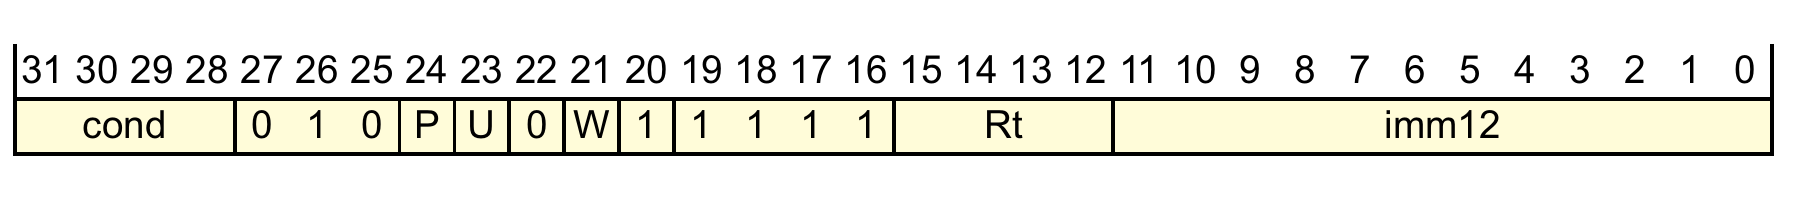
\includegraphics[width=\textwidth]{LDRliteral.png}\\
\hspace*{1mm}  1 1 1 0 \hspace*{5mm} 0  1  0 \hspace*{3mm} 1 \hspace*{2mm}1 \hspace*{2mm}0 \hspace*{1.5mm}0 \hspace*{1.5mm}1 \hspace*{3mm}1 1 1 1 \hspace*{6mm} 0 1 1 1 \hspace*{12mm}0 0 0 0 1 1 0 1 1 0 0\\
\vspace{0.1cm}
Vemos que Rt es 7 (R7)  y el valor imm12 = 0x06C es lo que debe sumarse al valor actual del PC para encontrar el literal que se cargará en R7.\\
 \end{textblock*}
\end{frame}

\begin{frame}{Accesorias del compilador / ensamblador}
 \begin{textblock*}{\textwidth}(.3cm,1.2cm)
  \begin{itemize}[<+->] \justifying \parskip 0.2cm
   \item El programa objeto generado ya sea con un compilador o con un ensamblador, tiene indefectiblemente un encabezado, precedente al código binario.
   \item Este encabezado es insumo fundamental del linker editor.
   \item En dicho encabezado, el ensamblador en este caso guarda el o los literal pools en la tabla de símbolos reubicables, de modo que el linker al armar la imagen del programa ejecutable los pueda terminar de ubicar combinándolos eventualmente con los literales de los restantes objetos que componen el proyecto.
  \end{itemize}
 \end{textblock*}
\end{frame}

\subsection{Loops y Branches}
\begin{frame}{Lo inevitable}
 \begin{textblock*}{\textwidth}(.3cm,1.2cm)
  \begin{itemize}[<+->]\justifying \parskip 0.2cm
   \item Son un mal necesario
   \item pero inevitable
   \item En algún momento necesitamos discontinuar el flujo de ejecución
   \begin{itemize}
    \item Por una interrupción
    \item Por invocar a una función
    \item Porque evaluada una condición hay que continuar por otra dirección
    \item Por estricta necesidad
   \end{itemize}
  \end{itemize}
 \end{textblock*}
\end{frame}

\begin{frame}[fragile]{Tipos de salto}
 \begin{textblock*}{\textwidth}(.3cm,1.2cm)
  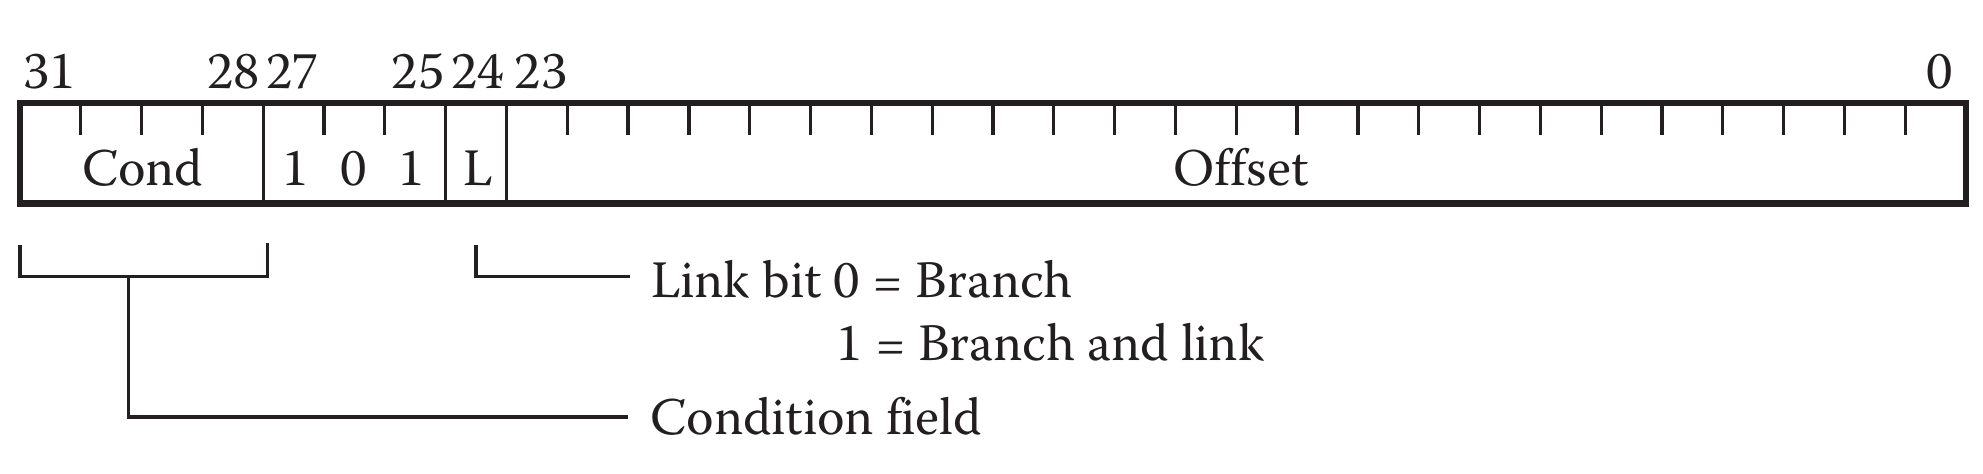
\includegraphics[width=\textwidth]{Branch.png}\\
  Tanto para B como BL, o BX, la cuestión es que se puede saltar alrededor de $2^{24}$ bytes del valor del Program Counter al momento de ejecutar el salto.\\
  Esto significa que el PC está apuntando a la instrucción sucesora secuencial del salto.\\
  \texttt{\textbf{Ej:}}\\
  \begin{lstlisting}[escapechar=\@, basicstyle=\scriptsize]
 b  DESTINO_ADDR
 add R1,R2,R6    /*Intrucci@\color{purple}\'o@n sucesora secuencial*/
  \end{lstlisting}
 \vspace{-0.4cm}
 Si DESTINO\_ADDR \textgreater $2^{24}$, entonces se arma en un literal pool
 \end{textblock*}
\end{frame}

\begin{frame}[fragile]{Saltos condicionales}
 \begin{textblock*}{\textwidth}(.3cm,1.2cm)
  \begin{footnotesize}
   \begin{center}
    \begin{tikzpicture}
     \node (tbl) {
     \rowcolors[]{1}{}{gray!5}
     \begin{tabularx}{\textwidth}{p{.18\textwidth} p{.21\textwidth} p{.38\textwidth} p{.15\textwidth} }
 \textbf{\color{white} Mnemónico} & \textbf{\color{white} Flag} & \textbf{\color{white} Significado} & \textbf{ \color{white} Código}\\
  EQ &  Z=1 & Equal & 0000\\
  NE &  Z=0 & Not Equal & 0001\\
  CS/HS &  C=1 & $\geq$ No Signado  & 0010\\
  CC/LO &  C=0 & $<$ No Signado& 0011 \\
  MI &  N=1 & Negativo & 0100 \\
  PL &  N=0 & Positivo o Cero & 0101\\
  VS &  V=1 & Overflow & 0110\\
  VC &  V=0 & No Overflow & 0111\\
  HI &  C=1, Z=0 & $>$ No Signado & 1000\\
  LS &  C=0, Z=1 & $\leq$ No Signado & 1001\\
  GE &  $N \geq V$ & $\geq$ Signado & 1010\\
  LT &  $N \neq V$ & $<$Signado & 1011\\
  GT &  Z=0, N=V & $>$Signado & 1100\\
  LE &  Z=1, $N \neq V$ & $\leq$Signado & 1101\\
  AL & Siempre & Default & 1110\\
     \end{tabularx}
     };
     \begin{pgfonlayer}{background}
     \draw[rounded corners,top color=red,bottom color=black,draw=white] ($(tbl.north west)+(0.14,0)$) rectangle ($(tbl.north east)-(0.13,0.45)$);
     \draw[rounded corners,top color=white,bottom color=black, middle color=red,draw=blue!20] ($(tbl.south west)+(0.12,0.5)$) rectangle ($(tbl.south east)-(0.12,0)$);
     \draw[top color=blue!1,bottom color=blue!20,draw=white] ($(tbl.north east)-(0.13,0.6)$) rectangle ($(tbl.south west)+(0.13,0.2)$);
     \end{pgfonlayer}
    \end{tikzpicture}
   \end{center}
  \end{footnotesize}
 \end{textblock*}
\end{frame}

\begin{frame}{Loops}
 \begin{textblock*}{\textwidth}(.3cm,1.2cm)
  \begin{itemize}[<+->]\justifying \parskip 0.3cm
   \item Trabajan con los saltos condicionales.
   \item CBZ y CBNZ Comparan y saltan si el registro operando es cero, o no es cero respectivamente. Útiles en loops.
  \end{itemize}
 \end{textblock*}
\end{frame}

\begin{frame}{Conclusiones}
 \begin{textblock*}{\textwidth}(.3cm,1.2cm)
  \begin{itemize} \justifying \parskip 0.3cm
   \item Hay instrucciones aritméticas, lógicas, de comparación, etc
   \item La mejor (y única) manera de aprenderlas es experimentando
   \item Hay Hojas de ayuda para tener un panorama rápido del set de instrucciones y poder luego buscar en la documentación los detalles (ruta recomendada)
  \end{itemize}
 \end{textblock*}
\end{frame}

\end{document}

